\documentclass[a4paper,12pt]{article}
\usepackage{template}
\usepackage{textcomp}
\usepackage{rotating}% in ph_thermodynamik.tex
\usepackage{booktabs}% for more beautiful hlines
\usepackage{multirow}% in ph_1wellen

\begin{document}
%W�rmestrahlung, Allgemeines zu Wellen
\section{Grundlagen der QM}
\subsection{Schwarzk�rperstrahlung}
\begin{tabular}{p{4cm} p{15cm}}
Schwarzer K�rper	& \begin{itemize}
				\item Ein sK absorbiert elektromagnetische Strahlung vollst�ndig. Somit (wegen Kirchhoffschem Strahlungsgesetz) ist sein Emissionsverm�gen im Vergleich zu beliebigen K�rper maximal ($\epsilon = 1$)
				\item Ein sK l�sst keine Strahlung hindurch und spiegelt oder streut nichts.
				\item Ein beliebiger K�rper kann bei keiner Wellenl�nge mehr Strahlung aussenden als ein sK
                	  \end{itemize}\\
Wiensches Verschiebungsgesetz	& \begin{tabular}[t]{l}
                             	   $\boxed{\lambda_{max} \cdot T = 2.898\cdot 10^{-3} \text{m K}}$\\
				   $[\lambda_{max}] = \mu m$; Wellenl�nge bei der die gr�sste Strahlungsintensit�t auftritt.\\
				   $[T] =$ K; absolute Temperatur der strahlenden Fl�che
				  \end{tabular}\\
Stefan-Boltzmann-Gesetz	& \begin{tabular}[t]{l}
                        	   $\boxed{P = \sigma A \epsilon T^4}$\\
				   $[P] =$ W; Leistung, die auf eine Seite von der Fl�che $A$ abgestrahlt wird.\\
				   $\sigma = 5.67\cdot 10^{-8} \tfrac{W}{m^2K^4}$, Stefan-Boltzmann-Konstante\\
				   $\epsilon \leq 1:$ Emissionsverm�gen
			  \end{tabular}\\
Planck'sches Strahlungsgesetz	& \begin{tabular}[t]{l}
                             	   $\boxed{\rho_E(\nu)d\nu = \frac{8\pi h\nu^3}{c^3}\frac{1}{e^{h\nu/k_B T}-1}d\nu}$\\
				   $\rho_E(\nu)d\nu:$ Volumendichte der thermischen Strahlung in einem Frequenzintervall $[\nu, \nu + \delta\nu]$\\
				   $[\nu] = $s$^{-1}$; Frequenz\\
				   $\rho_E(\lambda)d\lambda = \frac{8\pi hc}{\lambda^5}\frac{1}{e^{hc/\lambda k_B T}-1} d\lambda$
                             	  \end{tabular}\\
\end{tabular}
\subsection{Ebene Welle}
\begin{tabular}{p{4cm} p{7cm} p{8cm}}
Definition		& \multicolumn{2}{l}{$\vec A(\vec r,t) = \operatorname{Re}\left(\vec A_0 e^{ i\left(\vec k\cdot \vec r-\omega t\right)}\right) = \vec A_0 \cos(\vec k\cdot\vec r - \omega t)$}\\
Amplitude		& $\vec A_0$	& Dimension i.A. w�hlbar\\
Wellenvektor		& $\vec k$	&\\
Wellenzahl		& $k = | \vec k | = \frac{2\pi}{\lambda}$	& m$^{-1}$\\
Wellenl�nge		& $\boldsymbol{\lambda = \frac{2\pi}{k}}$	& $m$\\
Kreisfrequenz		& $\omega = 2\pi\nu$ Dispersionsrelation	& s$^{-1}$\\
Frequenz		& $\boldsymbol{\nu = \frac{\omega}{2\pi}}$	& s$^{-1}$\\
Periode			& $T = \frac{1}{\nu} = \frac{2\pi}{\omega}$	& s\\
Phasengeschwindigkeit	& $\boldsymbol{c = \frac{\omega}{k} = \lambda\nu }= \frac{\lambda}{T}$	& m s$^{-1}$\\
Gruppengeschwindigkeit	& $v_G = d\omega / dk$				&  m s$^{-1}$\\
Phase			& $\phi = \vec k \cdot \vec r -\omega t$	& dimensionslos\\
\end{tabular}
\begin{tabular}{p{4cm} p{4cm} p{11cm}}
Abh�ngigkeit von Medium	& \multicolumn{2}{p{15cm}}{Beim �bergang in ein Medium mit Brechungszahl $n = \sqrt{\mu_r \epsilon_r}$ �ndern sich folgende Gr�ssen wie folgt:}\\
			& Frequenz:	& $\nu \rightarrow \nu$\\
			& Wellenl�nge:	& $\lambda \rightarrow \frac{\lambda}{n}$\\
			& Lichtgeschwindigkeit:	& $c \rightarrow \frac{c}{n}$\\
			& Wellenzahl:	& $k \rightarrow k \cdot n$
\end{tabular}
\begin{tabular}{p{4cm} p{15cm}}
Schwebung	& \begin{tabular}[t]{ll}
         	  $E_0 \cdot e^{i(\omega_1 t)} + E_0 \cdot e^{i(\omega_2 t)} = 2E_0 \cos\left( \frac{\Delta\omega}{2} t \right) e^{i\bar{\omega}t}$	& \multirow{3}{*}{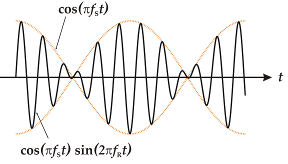
\includegraphics[width = 5cm]{ph_schwebung.png}}\\
		  $\Delta\omega = \omega_1 - \omega_2$\\
		  $\bar{\omega} = \frac{\omega_1 + \omega_2}{2}$
         	  \end{tabular}
		  \\
Beugung		& \begin{tabular}[t]{ll}
		   \multicolumn{2}{l}{$d$ = Breite des Spalts}\\
       		   $d \gg \lambda$	& Keine Beugung\\
		   $d \leq \lambda$	& Welle wird um Spalt gebeugt
       		  \end{tabular}\\
Interferenz	& \begin{tabular}[t]{ll}
           	   Maxima	& $d \sin \theta_m = m\lambda,\quad m = 0,1,2...$\\
		   Minima	& $d \sin \theta_m = (m-\tfrac{1}{2})\lambda,\quad m = 1,2,3,...$\\
		   Intensit�t	& $I = \frac{\sin^2 pz}{\sin^2 z}\quad z = \frac{\pi d}{\lambda}\sin\alpha$ p = \# Spalten
           	  \end{tabular}\\
\end{tabular}
\subsection{Wellenpakete}
Ein Wellenpaket ist eine �berlagerung von ebenen Wellen mit unterschiedlicher Frequenz aber gleicher Phase. Phasengleich bedeutet, dass verschiedene Wellen an einem Punkt $(x,t)$ den gleichen Wert haben.\\
\begin{tabular}{p{9.5cm} |p{9.5cm}}
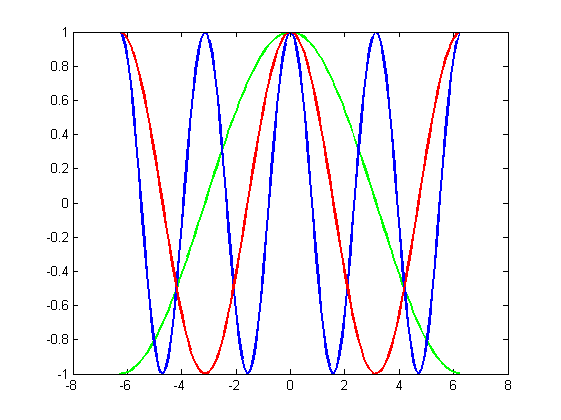
\includegraphics[width = 7cm]{ph_phasengleichewelle.png}	& 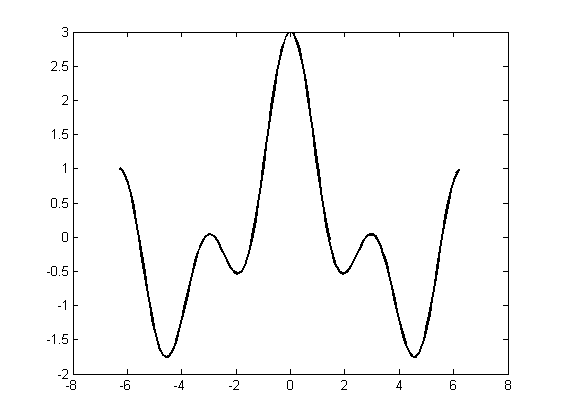
\includegraphics[width = 7cm]{ph_wellenpaket.png}\\
Phasengleiche (um x=0) Cosinusfkt. mit Wellenl�ngen $4\pi$, $2\pi$ und $\pi$	& �berlagerung: $\cos \tfrac{1}{2} x + \cos x + \cos 2x$\\
\end{tabular}\\
\begin{tabular}{p{4cm} p{15cm}}
allgemeinste Lsg. der SG	& $\Psi(x,t) = \sum_n c_n \psi_n(x)e^{-iE_nt/\hbar}\quad\psi_n$ sind L�sungen der SG.\\
Alternative Darstellung		& $\Psi(x,t) = \int g(k)\psi_k(x,t) dk\quad g(k)$ ist eine Gewichtungsfunktion.\\
\multicolumn{2}{p{19cm}}{Der Zusammenhang zwischen einer einzelnen Welle mit bekannter Frequenz und einem Wellenpaket kann auch mittels Fouriertransformation ausgedr�ckt werden:}\\
Welle				& $E(z,t) = F^{-1}\left\lbrace \tilde{E}(z,\omega)\right\rbrace = \frac{1}{2\pi}\int \tilde{E}(z,\omega)e^{i\omega t} d\omega$\\
Frequenzspektrum		& $\tilde{E}(z,\omega) = F\left\lbrace E(z,t) \right\rbrace = \int E(z,t)e^{-i\omega t} dt$\\
FWHM (Full width @ half maximum)	& Sei $f(x_1) = f(x_2) = \frac{1}{2}f(x_\mathrm{max})$ Dann ist FWHM = $|x_1-x_2|$\\
\end{tabular}
\subsubsection{Unterschied Wellenpaket - Welle in Bezug auf Unbestimmtheitsrelation}
\begin{enumerate}
\item Die Eigenzust�nde (Wellenfkt.) sind L�sungen f�r eine genau definierte Energie $\Rightarrow$ Ort ist unbestimmt (Unsch�rfrelation)
\item Durch Superposition mehrerer benachbarter Eigenzust�nde erh�lt man einen Puls, (der mit der Eigenfrequenz hin und her schwingt) und dessen Ort immer genauer bestimmbar wird.
\end{enumerate}


%Welle-Teilchen-Dualismus, de Broglie Wellenl�nge
\subsection{Photoelektrischer Effekt}
\begin{tabular}{p{4cm} p{15cm}}
	  & \begin{tabular}[t]{l}
	    $\boxed{E_{kin,max} = \left(\tfrac{1}{2} mv^2 \right) = h\nu - \Phi_0}$\\
	    $E_{kin,max}:$ maximale kinetische Energie der austretenden Elektronen\\
	    $\Phi_0:$ Austrittsarbeit: Mindestenergie um ein Elektron herauszul�sen.
	    \end{tabular}\\
Grenzfrequenz	& $E_{kin,max} > 0 \Leftrightarrow h\nu_0 > \Phi_0 \Leftrightarrow \nu_0 > \frac{\Phi_0}{h}$
\end{tabular}
\subsection{Compton Effekt und Photonen}
\begin{tabular}{p{4cm} p{15cm}}
Nichtrelativistische Energie	& $E = \frac{p^2}{2m}$\\
Relativistische Energie	& $E = m(v)c^2 = c\sqrt{m_0^2c^2 + p^2}$\\
Geschw. abh�ngigkeit	& $m(v) = m_0 \cdot \frac{1}{\sqrt{1-\tfrac{c^2}{v^2}}}$\\
Photonen im Vakuum	& \begin{tabular}[t]{ll}
		   Ruhemasse	& $m_0 = 0$\\
        	   Energie	& $E = h\nu = \frac{hc}{\lambda} = cp\quad$ (nur f�r Teilchen mit $m_0 = 0$!!)\\
		   Impuls	& $p = \frac{h}{\lambda}$\\
		   Ausbreitungsgeschwindigkeit	& $c$
        	  \end{tabular}\\
Compton Effekt		& \begin{tabular}[t]{p{14cm}}
              		   $\Delta \lambda = \lambda_2 - \lambda_1 = \frac{h}{m_e c} (1-\cos\varphi)$\\
			   $\frac{h}{m_e c} =: \lambda_{\text{Compton}} = 2.426 \cdot 10^{-12}$m\\
			   $\lambda_1$: Wellenl�nge des Photons vor dem Stoss mit einem freien Elektron.\\
			   $\lambda_2$: Wellenl�nge nach dem Stoss.\\
			   $\varphi$: Winkel zwischen einfallendem Photon (Welle) und gestreutem Photon\\
			   Der Compton-Effekt hat nur dann einen merklichen Einfluss, falls $\Delta \lambda / \lambda_1$ gross ist, d.h. $\lambda_1$ muss im pm-Bereich liegen (R�ntgenstrahlen).
              		  \end{tabular}
\end{tabular}
\subsection{Welle-Teilchen Dualismus}
Elektromagnetische Strahlung breitet sich wie eine Welle aus, und wechselwirkt mit Materie wie ein Teilchen.\\
\begin{tabular}{p{4cm} p{15cm}}
Wellencharakteristiken:		& Transmission, Beugung, Reflexion, Interferenz\\
Teilchencharakteristiken:	& Absorption, Emission
\end{tabular}

\subsection{De Broglie-Hypothese}
Laut de Broglie haben auch Teilchen mit Ruhemasse $>$ 0 eine Wellenl�nge.\\
\begin{tabular}{p{4cm} p{15cm}}
Materiewellen	& \begin{tabular}[t]{ll}
                        Wellenl�nge	& $\lambda = \frac{h}{p}$\\
			nicht relativistischer Impuls	& $p = mv$\\
			relativistischer Impuls	& $p = \frac{m_0v}{\sqrt{1-(v/c)^2}}$\\
			Materiewelle	& $\Psi(z,t) = \Psi_0 e^{i(\omega t-kz)}\quad \omega = \frac{2\pi c}{\lambda}$
                  \end{tabular}
\end{tabular}
%Schr�dingergleichung, Potentialstufe, Tunneleffekt etc.
\section{Schr�dingergleichung}
\subsection{Allgemeines}
\begin{tabular}{p{4cm} >{$}p{15cm}<{$}}
``Herleitung'' der SG			& \begin{array}[t]{rl}
						& \Psi(x,t) = \Psi_0 \exp \left( \frac{i}{\hbar} (p_x x-Et) \right) \quad \text{(de Broglie)}\\
				\Rightarrow	& p_x \Psi(x,t) = -i\hbar \frac{\partial}{\partial x} \Psi(x,t)\\
				\Rightarrow	& E \Psi(x,t) = i\hbar \frac{\partial}{\partial t} \Psi(x,t)\\
						& \text{Via Korrespondenzprinzip gilt: $E = \frac{\hat{p}^2}{2m}$}\\
				\Rightarrow	& E \Psi(x,t) = \underbrace{i\hbar \frac{\partial}{\partial t}}_{E} \Psi(x,t) = \underbrace{\frac{-\hbar^2}{2m} \frac{\partial^2}{\partial x^2}}_{H} \Psi(x,t) = \frac{\hat{p}^2}{2m}\Psi(x,t)\\
						& \text{L�sungsansatz (Separation der Variablen): $\Psi(x,t) = \psi(x) \cdot \chi(t)$}\\
				\Leftrightarrow	& \psi(x) i\hbar \frac{\partial \chi(t)}{\partial t} = \chi(t) \cdot \frac{-\hbar^2}{2m} \frac{\partial^2}{\partial x^2} \psi(x)\\
				\Leftrightarrow	& \frac{i \hbar \dot{\chi(t)}}{\chi(t)} = \frac{-\hbar^2}{2m} \frac{\psi''(x)}{\psi(x)} = E\\
				\Rightarrow	& \text{ODE 1: } i\hbar \dot{\chi(t)} = E \chi(t) \Rightarrow \chi(t) = \exp(\frac{-i}{\hbar} Et)\\
						& \text{ODE 2: } \frac{-\hbar^2}{2m} \psi''(x) = E \psi(x)
                 			  \end{array}\\
allgemeine SG				& \hat{H} \Psi = \hat{E} \Psi\\
allg. zeitabh�ngige L�sung		& \psi(\mathbf{r},t) = \psi(\mathbf{r}) e^{-i\frac{E}{\hbar}t} = \psi(\mathbf{r})e^{-i\omega t}\\
Normierungsbedingung			& \int_{-\infty}^{\infty} |\Psi(x)|^2 dx = 1\\
Aufenthalts wahrscheinlichkeitsdichte	& P(x) = |\Psi(x)|^2\\
Delokalisation				& \text{vollst�ndige Delokalisation eines Teilchens, falls $P(x) = konst.$}\\
Heisenberg'sche Unsch�rferelation	& \Delta x \Delta p \geq \tfrac{1}{2} \hbar\\
Kommutator				& \left[\hat{A},\hat{B}\right] \equiv \hat{A}\cdot \hat{B} - \hat{B} \cdot \hat{A}\quad \text{Falls} \left[\hat{A},\hat{B}\right] = 0\Rightarrow \text{A und B gleichzeitig messbar}\\
Operatoren				& \begin{array}[t]{lll}
          				   \hat{r}	& \text{Orts-Operator}	& \hat{r} = (x,y,z)^T \\
					   \hat{p}	& \text{Impuls-Operator}	& \hat{p} = -i\hbar\nabla = -i\hbar (\partial / \partial x, \partial / \partial y , \partial / \partial z)^T\\
					   \hat{H}	& \text{Hamilton-Operator*}	& \hat{H} = \frac{\hat{p}^2}{2m} + E_p(\hat{r}) = -\frac{\hbar^2}{2m}\nabla^2 + E_p(\hat{r})\\
					   \multicolumn{3}{l}{\text{* f�r ein freies Teilchen im Potentialfeld}}
          				  \end{array}\\
\end{tabular}
\subsection{allgemeine L�sung f�r SG mit Potential}
\begin{tabular}{p{4cm} >{$}p{15cm}<{$}}
zeitunabh�ngige Schr�dingergleichung (1-dim)	& -\frac{\hbar^2}{2m}\frac{d^2\psi(x)}{dx^2} + E_{pot}(x)\psi(x) = E\psi(x)\\
L�sung der zeitunabh�ngigen SG		& \begin{array}[t]{ll}
						& \underbrace{\frac{-\hbar^2}{2m}}_{=: -C} \frac{\partial^2}{\partial x^2} \psi(x) = (E-E_{pot}) \psi(x)\\
						& \text{Ansatz: $\psi(x) = e^{ikx}$}\\
				\Rightarrow	&  Ck^2\cdot e^{ikx} = (E-E_{pot}) \cdot e^{ikx}\\
				\Leftrightarrow	& k = \pm\sqrt{\frac{E-E_{pot}}{C}} = \pm\sqrt{\frac{(E-E_{pot})\cdot 2m}{\hbar^2}}\\
				\Rightarrow	& \psi_k(x) = A_k e^{ikx} + B_k e^{-ikx}
                                      	  \end{array}\\
L�sung f�r $E_{pot} = 0$		& \psi_1(x) = Ae^{ikx} + Be^{-ikx}\quad k^2 = \frac{2mE}{\hbar^2}\\
L�sung f�r $E < E_{pot}$		& \psi_2(x) = Ce^{-\alpha x} + De^{\alpha x}\quad \alpha^2 = \frac{2m}{\hbar^2}(E_{pot}-E)\\
L�sung f�r $E > E_{pot}$		& \psi_3(x) = Ee^{i\alpha'x} + Fe^{-i\alpha' x}\quad \alpha'^2 = \frac{2m}{\hbar^2}(E-E_{pot})\\
Stetigkeitsbedingungen			& \psi_i = \psi_j \quad\text{und}\quad \frac{\partial \psi_i}{\partial x} = \frac{\partial \psi_j}{\partial x} \text{ f�r $x=0$}\\
Teilchenstromdichte			& v |A|^2\quad v = \frac{p}{m} = \frac{\hbar k}{m}\\
Transmissionskoeffizient		& \frac{k_C|C|^2}{k_A|A|^2}\\
Reflexionskoeffizient			& \frac{k_B|B|^2}{k_A|A|^2}\quad \text{ Bedeutung von A,B,C wie unten Bsp. Potentialstufe}\\
					& R + T = 1\\

\end{tabular}
\subsection{Spezifische Probleme}
\subsubsection{Potentialstufe}
\begin{tabular}{p{4cm} >{$}p{15cm}<{$}}
$E_{pot}$	& E_{pot} = \begin{cases} 0 & x < 0 \text{ (Bereich I)}\\ E_0 & x \geq 0 \text{ (Bereich II)}\end{cases}\\\midrule
allg. L�sung ($E < E_{pot}$)	& \begin{array}[t]{l}
      		  \psi_I(x) = Ae^{ikx} + Be^{-ikx}\quad k^2 = \frac{2mE}{\hbar^2}\\
		  \psi_{II}(x) = Ce^{-\alpha x} + De^{\alpha x}\quad \alpha^2 = \frac{2m}{\hbar^2}(E_{pot}-E)
      		  \end{array}\\
Stetigkeitsbedingungen	& \left.\psi_I\right|_{x=0} = \left.\psi_{II}\right|_{x=0} \quad\text{und}\quad \left.\frac{\partial \psi_I}{\partial x}\right|_{x=0} = \left.\frac{\partial \psi_{II}}{\partial x}\right|_{x=0}\\
Randbedingungen	& \lim_{x\to\infty} \psi_{II} < \infty \text{ (vgl. Normierungsbedingung)}\\
spez. L�sung	& \begin{array}[t]{ll}
            	  D = 0 \text{ (aus RB)}	&\\
		  B = \frac{(ik+\alpha)A}{ik-\alpha}	& C = \frac{2ikA}{ik-\alpha}
            	  \end{array}\\\midrule
allg. L�sung ($E > E_{pot}$)	& \begin{array}[t]{l}
      		  \psi_I(x) = Ae^{ikx} + Be^{-ikx}\quad k^2 = \frac{2mE}{\hbar^2}\\
		  \psi_{II}(x) = Ee^{i\alpha'x} + Fe^{-i\alpha' x}\quad \alpha'^2 = \frac{2m}{\hbar^2}(E-E_{pot})
      		  \end{array}\\
spez.L�sung	& \begin{array}[t]{ll}
            	  F = 0 \text{ (aus RB)}	&\\
		  B = \frac{(k-\alpha')A}{k+\alpha'}	& E = \frac{2kA}{k+\alpha'}
            	  \end{array}\\
Transmissionskoeffizient	& \frac{v_{II} |E|^2}{v_I |A|^2} = \frac{\alpha'}{k} \left(\frac{2k}{k+\alpha'}\right)^2\\
Reflexionskoeffizient		& \frac{v_I |B|^2}{v_I |A|^2} = \left(\frac{k-\alpha'}{k+\alpha'}\right)^2
\end{tabular}
\subsubsection{Potentialtopf (1D)}
\begin{tabular}{p{4cm} >{$}p{15cm}<{$}}
$E_{pot}$	& E_{pot} = \begin{cases} 0 & 0 < x < a \text{ Bereich I}\\ \infty & \text{ sonst (Bereich II)}\end{cases}\\
allg. L�sung	& \begin{array}[t]{l}
            	  \psi_I(x) = Ae^{ikx} + Be^{-ikx}\quad k^2 = \frac{2mE}{\hbar^2}\\
		  \psi_{II}(x) = 0
            	  \end{array}\\
Randbedigungen	& \psi_I(x=0) = \psi_I(x=a) = 0\\
spez. L�sung	& \psi_I(x) = \sqrt{\frac{2}{a}} \sin(kx)\quad k = \frac{n\pi}{a}\quad \Rightarrow \lambda = \frac{2\pi}{k}\\
Energieeigenwert	& E = \frac{\hbar^2 k^2}{2m} = \frac{n^2\pi^2\hbar^2}{2ma^2}
\end{tabular}
\subsubsection{Potentialtopf (3D)}
\begin{tabular}{p{4cm} >{$}p{15cm}<{$}}
SG in 3 Dimensionen			& \psi(x,y,z) = \psi_1(x)\psi_2(y)\psi_3(z)\quad\text{$\psi_{1,2,3}$ sind Wellenfkt. im 1-dim. Kasten}\\
Particle in a cube			& \begin{array}[t]{l}
                 			   \psi(x,y,z) = \sqrt{\frac{8}{a^3}} \sin(\tfrac{n_1\pi}{a} x) \sin(\tfrac{n_2\pi}{a} y) \sin(\tfrac{n_3\pi}{a} z)\\
					   E = \frac{\hbar^2 \pi^2}{2ma^2}(n_1^2+n_2^2+n_3^2)\\
                 			  \end{array}
\end{tabular}
\subsubsection{Der Tunneleffekt}
\begin{tabular}{p{4cm} p{15cm}}
Potentialstufe		& $V(x) = \begin{cases}
              		          0	& x < 0 \quad\text{Bereich A}\\
				  V	& 0 \leq x \leq D \quad\text{Bereich B}\\
				  0	& D < x \quad\text{Bereich C}
              		          \end{cases}$\\
SG			& \begin{tabular}[t]{l}
			    $\hat{H} \Psi_A(x) = -\frac{\hbar^2}{2m} \frac{d^2}{dx^2} \Psi_A(x) = E \Psi_A(x)$\\
			    $\hat{H} \Psi_B(x) = -\frac{\hbar^2}{2m} \frac{d^2}{dx^2} \Psi_B(x) + V \Psi_B(x) = E \Psi_B(x)$\\
			    $\hat{H} \Psi_C(x) = -\frac{\hbar^2}{2m} \frac{d^2}{dx^2} \Psi_C(x) = E \Psi_C(x)$
			  \end{tabular}\\
L�sungen		& \begin{tabular}[t]{ll}
			    $\Psi_A(x) = Ae^{ikx} + Be^{-ikx}$		& $k = \sqrt{\frac{2mE}{\hbar^2}}$\\
			    $\Psi_B(x) = A'e^{ik'x} + B'e^{-ik'x}$	& $k' = \sqrt{\frac{2m(E-V)}{\hbar^2}} = i\kappa$\\
			    $\Psi_C(x) = A''e^{ikx} + B''e^{-ikx}$
        		  \end{tabular}\\
Randbedingungen		& \begin{tabular}[t]{l}
			    $\Psi_A(0) = \Psi_B(0)$\\
			    $\frac{d}{dx} \Psi_A(0) = \frac{d}{dx} \Psi_B(0)$\\
			    $\Psi_B(D) = \Psi_C(D)$\\
			    $\frac{d}{dx} \Psi_B(D) = \frac{d}{dx} \Psi_C(D)$\\
			    $B'' = 0$ (keine reflektierte Komponente rechts der Barriere erlaubt)
			  \end{tabular}
\end{tabular}
Letztlich hat man nur 5 Randbedingungen f�r 6 Unbekannte. Man kann also lediglich die Tunnelwahrscheinlichkeit $P_T = \frac{|A''|^2}{|A|^2}$ angeben, indem man $A''$ durch $A$ ausdr�ckt. $P_T = \frac{4E(V-E)}{4E(V-E) + V^2\sinh^2(\kappa D)}$ Grunds�tzlich wird die Tunnelwahrscheinlichkeit klein f�r breite Barrieren ($D\to\infty$), hohe Barrieren ($V\to\infty$) und grosse Massen $m$

\subsubsection{QM harmonischer Oszillator}
Der QM harmonische Oszillator wird verwendet, um bspw. molekulare Vibrationsbewegungen zu modellieren.
\begin{tabular}{p{4cm} p{15cm}}
SG		& $\hat{H} \Psi = \left( -\frac{\hbar^2}{2m} \frac{d^2}{dx^2} + \frac{1}{2}kx^2 \right) \Psi = E\Psi$\\
Eigenwerte	& $E_n = (n + \frac{1}{2})\hbar\omega$\\
Eigenfunktionen	& $\Psi_n = N_nH_n(\sqrt{\alpha}x) e^{-\alpha x^2/2 }\quad \alpha = \frac{\sqrt{mk}}{\hbar}\quad H_n:$  Hermite-Polynome
\end{tabular}
\subsubsection{3D QM harm. Osz.}
\begin{tabular}{p{4cm} p{15cm}}
Eigenwerte	& $E_n = (n_x + n_y + n_z + \frac{3}{2})\hbar\omega$\\
Eigenfunktionen	& $\Psi_n = \Psi_{n_x} \cdot \Psi_{n_y} \cdot \Psi_{n_z}$
\end{tabular}
\subsection{Weiteres}
\begin{tabular}{p{4cm} >{$}p{15cm}<{$}}
Postulat \# 2 der QM			& \text{Einzig m�gliches Messresult einer physik. Gr�sse $A(\mathbf{r,p})$ ist ein Eigenwert $a_n$}\\
					& \text{von Operator $\hat{A}(\hat{\mathbf{r}},\hat{\mathbf{p}}) \Rightarrow \hat{A} \psi_n = a_n \psi_n$}\\
Postulat \# 3 der QM			& \text{WSK dass $a_n$ Messresultat ist,ist $|c_n|^2$, falls Zustand des Systems: $\Phi = \sum_n c_n\psi_n$}\\
Erwartungswert				& \langle A \rangle = \int \Psi^{\asterisk} \hat{A} \Psi dxdydz\\
Beispiel				& \text{(1-dim) Energieerwartungswert: } \langle E_{kin} \rangle = \int \Psi^{\ast} \hat{H} \Psi dx
\end{tabular}
%Bohr'sches Atommodell, QM Drehimpuls, QM Coulomb Potential
\section{Bohr'sches Atommodell}
\begin{tabular}{p{4cm}p{15cm}}
Quantisierung des Bahndrehimpuls	& $L_n = m_e v r_n = n\hbar$\\
diskrete Energiezust�nde		& $\Delta E = E_2 - E_1 = h\nu$\\
�bergangsfrequenz			& $\nu = \frac{\Delta E}{h}$\\
Absorption				& $A + h\nu \rightarrow A^{\ast}$\\
spontane Emission			& $A^{\ast} \rightarrow A + h\nu$ (inkoh�rente Strahlung, zuf�llig in alle Rtg.)\\
stimulierte Emission			& $A^{\ast} + h\nu \rightarrow A + 2 h\nu$ (koh�rente Strahlung)\\
Atomradien nach Bohr			& $r_n = \frac{n^2}{Z}a_0,\quad a_0 = 0.529 $\AA$,\quad n = 1,2,3,...,\quad Z = $ Kernladungszahl\\
zugeh�rige Energien			& $E_n = -13.606 eV \frac{Z^2}{n^2}$\\
Wasserstoffspektrum beim Energieniveau�bergang			& $\nu = RcZ^2\left( \frac{1}{n_1^2} - \frac{1}{n_2^2} \right)Hz,\quad n_2 > n_1, Z$ = Kernladungszahl\\
Rydberg-Konstante			& $R = 1.0973731534 \cdot 10^7 $m$^{-1}\quad Rc = 3.2899 \cdot 10^{15}$
\end{tabular}
\section{QM Drehimpuls}
\begin{tabular}{p{4cm} >{$}p{16cm}<{$}}
Drehimpulsoperator	&\hat{\mathbf{L}} = \hat{\mathbf{r}} \times \hat{\mathbf{p}} = -i\hbar
											\begin{pmatrix}
											y\frac{\partial}{\partial z} - z\frac{\partial}{\partial y}\\ 
											z\frac{\partial}{\partial x} - x\frac{\partial}{\partial z}\\ 
											x\frac{\partial}{\partial y} - y\frac{\partial}{\partial x}
											\end{pmatrix}\\
			&\hat{L_z} = -i\hbar \left( x\frac{\partial}{\partial y} - y\frac{\partial}{\partial x}\right) = -i\hbar\frac{\partial}{\partial\varphi}\\
			&\hat{\mathbf{L}}^2 = \hat{L}_x^2+\hat{L}_y^2+\hat{L}_z^2 = -\hbar^2 \Delta_{\theta,\varphi}\\
Kommutativit�t		&\langle L_z, \hat{\mathbf{L}}^2 \rangle = 0\qquad \langle L_z, L_x \rangle \neq 0 \neq \langle L_z, L_y \rangle \\
			&\Rightarrow \text{In der QM sind nur eine Komponente und Betrag des Drehimpuls unabh�ngig.}\\
Drehimpulsgleichungen	& \begin{array}[t]{|lrll|}
			  \hline
             		   \hat{\mathbf{L}}^2 ~ Y_{l,m_l}(\theta,\varphi) =	& l(l+1)\hbar^2	& Y_{l,m_l}(\theta,\varphi)	& l = 0,1,2,3,...\\
			   \hat{L}_z  ~ Y_{l,m_l}(\theta,\varphi) =		& m_l\hbar 	& Y_{l,m_l}(\theta,\varphi)	& m_l = -l,-l+1,...,l-1,l\\\hline
             		  \end{array}\\
Kugelfunktionen		& \begin{array}[t]{l}
               		   Y_{l,m_l}(\theta,\varphi) = C P_l^{|m_l|} (\cos \theta)e^{im_l\varphi}\\
			   P_n^m(z) \equiv \text{ Legendre-Polynome}\\
			   \text{L�sungen zu $Y_{l,m_l}$: Alonso-Finn S.134}
               		  \end{array}\\
Quantenzahlen		& \text{
			     \begin{tabular}[t]{llll}
			     Principal quantum number	& n & 1,2,3,... & unlimitiert\\
							&   & K,L,M,... &\\
			     Orbital quantum number	& l & 0,1,2,... n-1 & n m�gliche Werte\\
							&   & s,p,d,f,..    &\\
			     Orbital magntic quantum number & $m_l$ & -l, l+1,..., l-1, l& 2l+1 m�gliche Werte\\
			     Spin quantum number	& $m_s$  & $-\frac{1}{2},\frac{1}{2}$	& 2 m�gliche Werte\\
			     \end{tabular}
			   }
\end{tabular}
\section{QM Coulomb-Potential (Wasserstoffatom)}
\begin{tabular}{p{4cm} p{15cm}}
Schr�dingergleichung	& $\hat{H} = -\frac{\hbar^2}{2m_K} \nabla^2_K  -\frac{\hbar^2}{2m_e} \nabla^2_e - \frac{Ze^2}{4\pi\epsilon_0 r} +$ andere Terme\\
vereinfachte SG		& \begin{tabular}[t]{l}
               		  $\hat{H}\Psi = \left( -\frac{\hbar^2}{2\mu} \nabla^2_r - \frac{Ze^2}{4\pi\epsilon_0 r} \right) \Psi = E\Psi$ (QM Coulomb-Potential)\\
			  $\mu = \frac{m_e \cdot m_K}{m_e + m_K} \approx m_e$\\
			  $Z =$ Kernladungszahl
               		  \end{tabular}\\
Ansatz f�r Eigenfkt.	& $\Psi(r,\theta,\phi) = R(r) \cdot Y_{lm}(\theta,\phi)$\\
L�sungen		& \begin{tabular}[t]{lcll}
			  $R_{n,l}(r)$	& = & $N_{n,l} \exp \left\lbrace -\frac{Zr}{na} \right\rbrace \left( \frac{2Zr}{na} \right)^l L^{2l+1}_{n-l-1}\left( \frac{2Zr}{na} \right)$	&$n = 1,2,...$\\
			  \multicolumn{4}{l}{$a = \frac{m_e}{\mu}a_0;\quad a_0 = \frac{4\pi \epsilon_0 \hbar^2}{m_e e^2} = 0.0529$ nm;$\quad L:$ Laguerre-Polynome}\\
        		  $Y_{lm}$	& = & Eigenfkt. des Drehimpulsoperators		& $l = 1,...,(n-1)$\\
					&	&					& $m = -l,-l+1,...l$\\
			  \multicolumn{4}{l}{Superpositionen sind nat�rlich auch wieder L�sungen!}
        		  \end{tabular}\\
Energieeigenwerte	& \begin{tabular}[t]{l}
                 	  $E_{n,l,m} = E_n = -\frac{hcRZ^2}{n^2} = -13.606eV \frac{Z^2}{n^2}$\\
			  $c =$ Lichtgeschwindigkeit; $R =$ Rydberg-Konstante
                 	  \end{tabular}\\
Entartung		& $g = \sum_{l=0}^{n-1} (2l+1) = n^2$ (Pro $l$ gibt es $2l+1$ $m$ mit gleichem Energieeigenwert)\\
radiale WSKDichte	& \begin{tabular}[t]{ll}
                 	  WSKDichte		&$p_{n,l}(r) dr = |R_{n,l}(r)^2| r^2 dr$\\
			  Radius des Maximums	& $\arg\max_r p_{n,l}(r) = r_{pmax} = \frac{n^2}{Z}a$ (Bohr'scher Atomradius)\\
			  Mittlerer Radius	& $\frac{a}{2Z} \left(3n^2-l(l+1) \right)$
                 	  \end{tabular}
\end{tabular}
\section{Zeeman-Effekt}
Unter Einfluss eines Magnetfelds offenbaren sich ungeahnte Zusatzenergien, die f�r die Aufspaltung von entarteten Energiezust�nden sorgen.\\
\begin{tabular}{p{4cm} >{$}p{16cm}<{$}}
magnetisches Bahn-Dipolmoment	& \mu_L = -\frac{e}{2m_e}\mathbf{L}\\
z-Komponente		& \mu_{L,z} = -\frac{e\hbar}{2m_e}m_l\\
Bohr'sches Magneton	& \mu_B = \frac{e\hbar}{2m_e} = 9.2732 \cdot 10^{-24} = 5.6564 \cdot 10^{-5}eVT^{-1}\\
Zusatz-Energie durch Magnetfeld	& E_B = -\mu_L \cdot B = \frac{e}{2m_e}\mathbf{L\cdot B}\\
z-Achse parallel Rtg. Magnetfeld	& E_B = \mu_B B m_l\\
Drehmoment Elektron	& \tau = \mu_L \times B = -\frac{e}{2m_e} \mathbf{L\times B}
\end{tabular}
\section{Elektronenspin}
Motiviert z.B. durch Stern-Gerlach-Versuch oder auch Doubletts bei Wellenl�ngen, z.B. D-Linien von Natrium. Der Elektronenspin ist ein Zusatzspin, der sich zum Drehimpuls addiert.\\
\begin{tabular}{p{4cm} >{$}p{16cm}<{$}}
Gesamtdrehimpuls	& \mathbf{J = L+S}\\
Gesamtdrehmoment	& \mu = \mu_L + \mu_S = -\frac{e}{2m_e}(\mathbf{L}+g_S\mathbf{S})\\
Drehimpulsgleichungen	& \begin{array}[t]{|lrll|}
			  \hline
             		   \hat{\mathbf{S}}^2 ~ \chi_{s,m_s} =	& s(s+1)\hbar^2	& \chi_{s,m_s}	& s = \frac{1}{2}\\
			   \hat{S}_z  ~ \chi_{s,m_s} =		& m_s\hbar 	& \chi_{s,m_s}	& m_s = \pm \frac{1}{2}\\\hline
			   \multicolumn{4}{l}{\text{Die genaue Gestalt von $\chi$ ist Wurst.}}
             		  \end{array}\\
vollst�ndige WFkt.	& \Psi_{nlm_lm_s} = R_{nl}(r)Y_{lm_l}(\theta,\phi) \chi_{m_s}\\
Addition von Bahndrehimpuls und Elektronenspin	& j = \left| l\pm \frac{1}{2} \right| 
\end{tabular}
\section{Addition von Drehimpulsen}
Sei $\hat{\vec J} = \hat{\vec{j}}_1 + \hat{\vec{j}}_2$ der resultierende Drehimpuls.\\
\begin{tabular}{p{4cm} p{15cm}}
Zugeh�rige Quantenzahlen	& \begin{tabular}[t]{l}
                        	  $\hat{\vec{j}}_1: |j_1,m_1\rangle$\\
				  $\hat{\vec{j}}_2: |j_2,m_2\rangle$\\
				  $\hat{\vec{J}}: |J,M\rangle$\\
				  Zur Erinnerung: $m = \pm j, \pm (j-1), ...$
                        	  \end{tabular}\\
gekoppelte Darstellung		& $|j_1,m_1,J,M \rangle$: In der gekoppelten Darstellung setzt man die Quantenzahlen $J$ und $M$ fest. \\
Betrag und z-Komponente		& \begin{tabular}[t]{lcl}
				    $|\vec{J}| = \hbar \sqrt{J(J+1)}$	& $\Rightarrow $	& $|\vec{J}| = |\vec{j_1} + \vec{j_2}| = ??$\\
				    $J_z = \hbar M$			& $\Rightarrow $	& $J_z = j_{1,z} + j_{2,z} = \hbar(m_1 + m_2)$
				  \end{tabular}\\
\multicolumn{2}{l}{$M$ ist immer gleich $m_1 + m_2$. Weil $|M| \leq |J|$ sein muss, k�nnen wir die m�glichen Werte f�r $J$ aus $M$ ableiten.}\\
Resultierende Quantenzahlen	& \begin{tabular}[t]{|l|}
				  \hline
                           	  $J = j_1 + j_2, j_1 + j_2 - 1,..., |j_1-j_2|$ \\
				  $M = m_1 + m_2$\\\hline	
                           	  \end{tabular}\\
Bra-Ket Notation		& $|j_1,j_2,J,M\rangle$\\
Anzahl Basisfunktionen		& $\underbrace{(j_1+j_2)}_{\text{\# J-Werte}} \cdot \underbrace{(2(j_1+j_2) + 1)}_{\text{\# M-Werte pro J-Wert}}$\\
Addition von Elektronenspin und Bahndrehimpuls	& Sei $\vec{j}_1 = \vec{L}$ und $\vec{j}_2 = \vec{S}$. Wir wissen, dass $m_s = \pm \frac{1}{2} \Rightarrow j_2 = \frac{1}{2}$, wogegen $m_l = \pm l, \pm (l+1), ... \Rightarrow j_1 = l \quad(l = 0,1,2,...,n-1)$. Somit sind die m�glichen Werte f�r $J$: $l+\frac{1}{2}$ und $l-\frac{1}{2}$. Dies entspricht den F�llen parallel und antiparallel. Der Elektronenspin kann relativ zum Bahndrehimpuls also nur zwei m�gliche Orientierungen haben. Ausnahme: F�r $j_1 = l = 0$ ist $j_1 + j_2 = |j_1 - j_2|$, somit kann $J$ nur einen Wert haben.
\end{tabular}
%QM Atome mit vielen Elektronen
\section{Atome mit vielen Elektronen}
\begin{tabular}{p{4cm} p{15cm}}
Ein Protonen, zwei Elektron System	& $E_{pot} = -\frac{Ze^2}{4\pi\epsilon_0 r_1} -\frac{Ze^2}{4\pi\epsilon_0 r_2} + \underbrace{\frac{e^2}{4\pi\epsilon_0 r_{12}}}_{Elektron-Elektron-Abstossung}$\\
Modell abgeschirmtes Zentralfeld	& $E = 2(Z-\delta)^2 E_H\quad E_H = -13.6 eV, \delta =$ Abschirmungskonstante\\
Bahnwellenfunktion Atom			& $\Psi_{Atom}(2,1) =  \Psi_a(2)\Psi_b(1) \pm \Psi_a(1) \Psi_b(2) = \pm \Psi_{Atom}(1,2)\quad$ a,b: Zust�nde; 1,2: Elektronen\\
symmetrische Bahnwellenfunktion		& $\Psi_S(1,2) = \Psi_S(2,1)\quad \lim_{a\to b} \Psi_S > 0$\\
					& $\Rightarrow$ Elektronen k�nnen einander nahe kommen $\Rightarrow$ Hohe mittlere Abstossungsenergie\\
antisymmetrische Bahnwellenfkt.		& $\Psi_A(1,2) = -\Psi_A(2,1)\quad \lim_{a\to b} \Psi_A = 0$\\
					& $\Rightarrow$ Elektronen sind einander nie nahe $\Rightarrow$ Niedrige mittlere Abstossungsenergie\\
gleiche Zust�nde			& Die Zust�nde $a,b$ entsprechen Quantenzust�nden $n,l,m_l$. Sind zwei Elektronen im gleichen Zustand, so ist die antisymmetrische Bahnwellenfkt. $\Psi_A(1,2) = \Psi_a(2)\Psi_a(1) - \Psi_a(1)\Psi_a(2) = 0$ und somit nicht erlaubt.\\
Spins				& Die Spins der beiden Elektronen betragen jeweils $\frac{1}{2}$. Je nach Orientation (parallel, antiparallel) k�nnen sie sich zu 0 oder 1 addieren\\
Spinwellenfkt			& Zur Erinnerung: $\chi_+$ bezeichnet die Spinwellenfkt bzgl. $m_s = \tfrac{1}{2}$, $\chi_-$ diejenige bzgl. $m_s = -\tfrac{1}{2}$\\
Gesamtspin $S=0$ (Singluett)	& $\chi_A = \chi_+(1)\chi_-(2)-\chi_+(2)\chi_-(1)\quad M_S = 0$ antisymmetrische Spin-Wellenfkt\\
Gesamtspin $S=1$ (Triplett)	& \begin{tabular}[t]{ll}
                           	   $\chi_S = \chi_+(1)\chi_+(2)$	& $M_S = 1$\\
				   $\chi_S = \chi_+(1)\chi_-(2) + \chi_+(2)\chi_-(1)$	& $M_S = 0$\\
				   $\chi_S = \chi_-(1)\chi_-(2)$	& $M_S = -1$
                           	  \end{tabular} symmetrische Spin-Wellenfkt.\\
Gesamtwellenfunktion		& \begin{tabular}[t]{p{14cm}}
                    		  $\Psi_{Gesamt} = $ Bahnwellenfkt $\cdot$ Spinwellenfkt = f�r Fermionen immer ANTIsymmetrisch, f�r Bosonen immer symmetrisch. Weil Elektronen Fermionen sind, m�ssen Gesamtwellenfkt. von Atomen immer antisymmetrisch sein.\\
				  Singuletts: symmetrische Bahnwfkt $\cdot$ antisymmetrische Spinwfkt.\\
				  Tripletts: antisymmetrische Bahnwfkt $\cdot$ symmetrische Spinwfkt.
                    		  \end{tabular}\\
				& 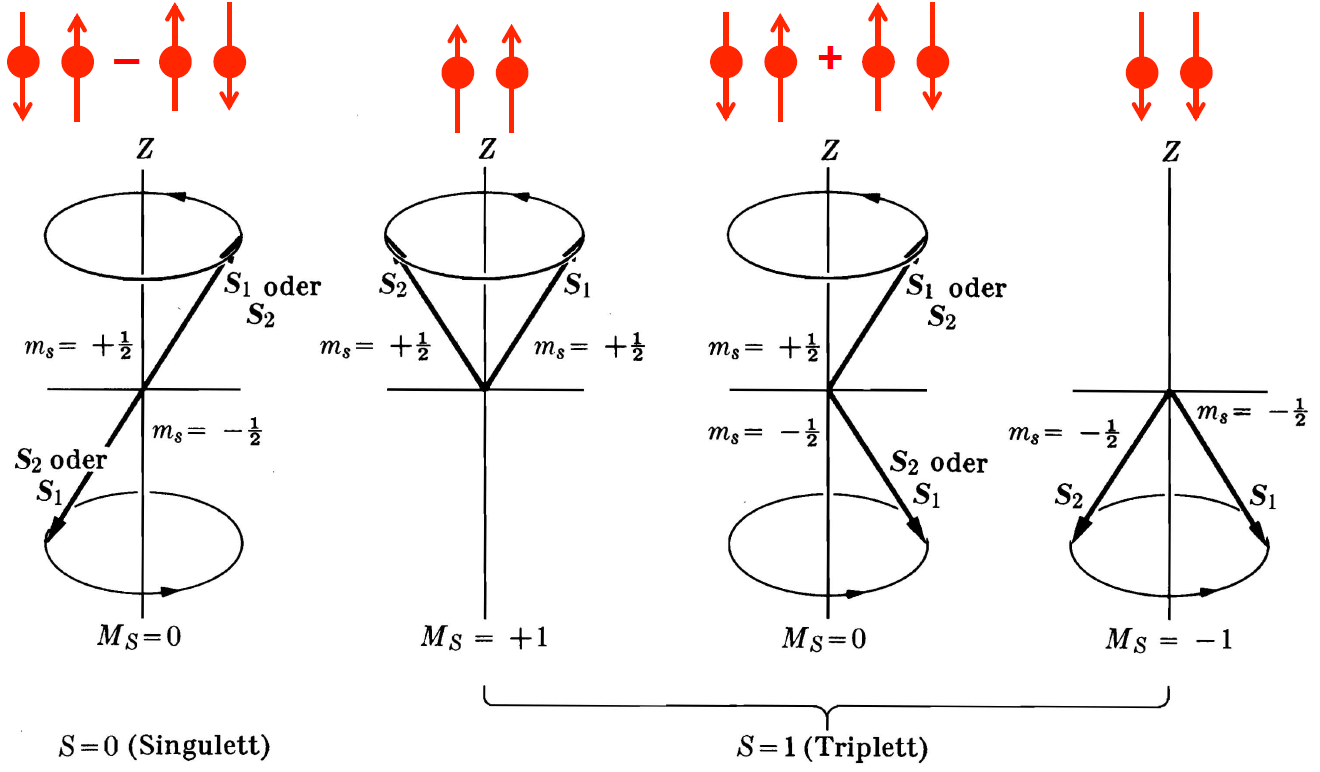
\includegraphics[width = 15cm]{ph_spin.png}\\
\end{tabular}\newpage
\begin{tabular}{p{4cm} p{15cm}}
Anzahl versch. Wellenfkt.	& Ein Zwei-Teilchen System mit je $n$ verschiedenen Zust�nden hat $\tfrac{1}{2} n(n+1)$ symmetrische und $\tfrac{1}{2} n(n-1)$ antisymmetrische Zust�nde. Dies gilt selbstverst�ndlich f�r Bahn- und Spinwellenfkt. Merke: Ein Teilchen mit Spin $S$ hat $n = 2S+1$ versch. Zust�nde\\
Ausschliessungsprinzip		& Jeder Quantenzustand $(n,l,m_l,m_s)$ kann h�chstens von einem Elektron (allg. Fermionen) eingenommen werden. Die Anzahl Zust�nde ist somit beschr�nkt durch die Abh�ngigkeiten der Quantenzahlen.\\
Regel von Hund			& Im Grundzustand von Atomen hat der resultierende Spin den gr�sstm�glichen Wert, der mit dem Ausschliessungsprinzip vereinbar ist\\
Elektronenkonfiguration		& $\text{(Hauptquantenzahl)(Bahndrehimpuls)}^{\text{Anz.Elektronen}}\quad $ Bsp: $1s^2 2s^2 2p$ 5$e^- \Rightarrow$ Bor\\
Besetzungszahl (max. \# $e^-$)	& 2(2l+1)\\
Auswahlregeln (Atom�berg�nge) 	& \begin{tabular}[t]{l}
             		  Emission und Absorption von Photonen:\\
			  $\Delta l = l_f - l_i = \pm 1$\\
			  $\Delta j = j_f - j_i = 0, \pm 1\quad j_i = 0 \Rightarrow j_f \neq 0$
             		  \end{tabular}\\
\end{tabular}


%QM Molek�le
\section{Molek�le}
LCAO-Approximation: Linear Combination of Atomic Orbitals.
\subsection{$H_2^+$ Molek�l (ein Elektron, zwei Protonen)}
\begin{tabular}{p{4cm} p{15cm}}
Hamilton-Operator	& $\hat H = -\frac{\hbar^2}{2m} \nabla^2 + \frac{e^2}{4\pi\epsilon_0} \left(-\frac{1}{r_1}- \frac{1}{r_2} + \frac{1}{r} \right)$ $r$: Abstand Proton-Proton, $r_{1,2}$: Abstand Elektron-Proton\\
LCAO-Approximation	& Spalte $H_2^+$ gedanklich auf in $H$ und $H^+$, dann gibt es eine Wellenfunktion $\Psi_1$, bei der das $H$ links ist und eine Wellenfunktion $\Psi_2$, bei der das $H$ rechts ist. Diese aufgespaltenen Zust�nde bringt man durch Linearkombination wieder zusammen.\\
Gesamtwellenfkt.	& \begin{tabular}[t]{l}
                	   $\Psi_{gerade} = \Psi_1 + \Psi_2$\\
			   $\Psi_{ungerade} = \Psi_1 - \Psi_2$\\
			   $\Rightarrow$ Durch die �berlappung (LCAO) entstehen zwei Molek�lorbitale
                	  \end{tabular}\\
Mittlere Energie des Elektrons	& $E = \frac{\int \Psi^{\asterisk} H \Psi dV}{\int \Psi^{\asterisk} \Psi dV} = E_a + \frac{e^2}{4\pi\epsilon_0 r} - \frac{A\pm B}{1\pm S}\quad +: \Psi_{gerade}, -:\Psi_{ungerade}$\\
�berlappintegral (Proton-Proton)	& $S = S(r) = \int \Psi(r_1) \Psi_2(r_1)dV_1\quad \lim_{r\to 0} S = S_{max}$\\
Anziehungsenergie (Elektron-Proton 2)	& $A = A(r) = \frac{e^2}{4\pi\epsilon_0}\int \frac{\Psi_1^2(r_1)}{r_2}dV_1$\\
�berlappungsterm (Elektron-Proton 1)	& $B = B(r) = \frac{e^2}{4\pi\epsilon_0} \int \frac{\Psi_1(r_1)\Psi_2(r_2)}{r_1}dV_1$\\
Kovalente Bindung	& $\Psi_1 + \Psi_2$ ist bindend und macht die kovalente Bindung. $\Psi_1 - \Psi_2$ ist dagegen nichtbindend.\\
			& 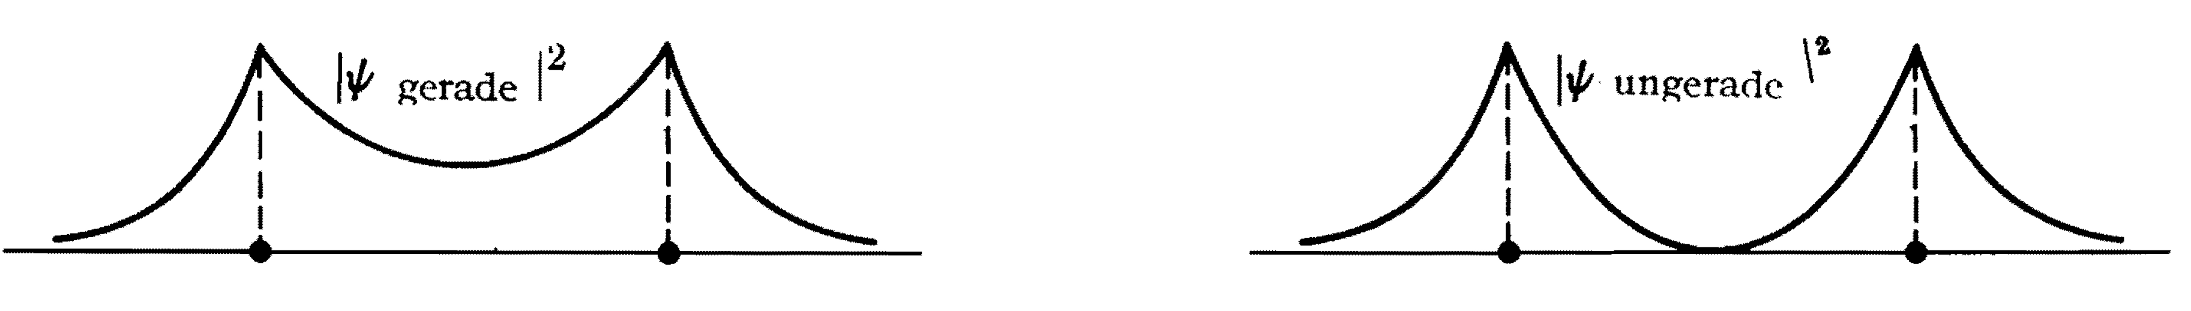
\includegraphics[width = 14cm]{ph_kovalentebdg.png}
\end{tabular}
\subsection{$H_2$ Molek�l (zwei Elektronen, zwei Protonen)}
Das Ganze funktioniert im Prinzip analog, nur dass man jetzt Atomorbitale linear kombiniert.\\
\begin{tabular}{p{4cm} p{15cm}}
Pauli-Prinzip	& Da wir mehr als ein Elektron haben, muss die Gesamtwellenfkt. antisymmetrisch sein.\\
Drehimpuls	& Drehimpuls $L$ eines $e^-$ nicht konstant, da kein Zentralfeld (lineares Molek�l)\\
		& $L_z = m_l\hbar$ konstant, da Kraft auf Elektronen immer durch Protonenachse\\
Drehimpulszust�nde im Molek�l	& \begin{tabular}[t]{lcccc}
                             	   $m_l$		& 0        & $\pm$ 1 & $\pm$ 2  & $\pm$ 3\\
				   Symbol		& $\sigma$ & $\pi$   & $\delta$ & $\Phi$\\
				   $\# e^-$		& 2	   & 4	 & 4	  & 4\\
				   \multicolumn{5}{l}{$\# e^-$ wegen Spin up, down}
                             	  \end{tabular}\\
LCAO		& Nun werden Atomorbitale analog zu oben linear kombiniert. Das resultierende MO h�ngt von den $m_l$ der Elektronen in den Atomorbitalen ab.\\
Beispiele	& 2 ns Atomorbitale ergeben ein $\sigma$ Molek�lorbital, weil $m_l = 0$ f�r ns Atomorbitale\\
		& 2 np Atomorbitale ergeben entweder ein $\sigma$ MO ($np_z$) oder ein $\pi$ MO ($np_x, np_y$), da $m_l$ f�r die p-AO -1,0,1 ist.\\
gerade, ungerade	& Subscript g: gerade Wellenfunktion (= MO), Subscript u: ungerade, Bsp: $\sigma_u$\\
bindend, nichtbindend	& Superscript $\ast$: nichtbindende Wellenfunktion (= MO), Bsp: $\sigma_u^{\ast}$\\
Elektronenkonfiguration	& 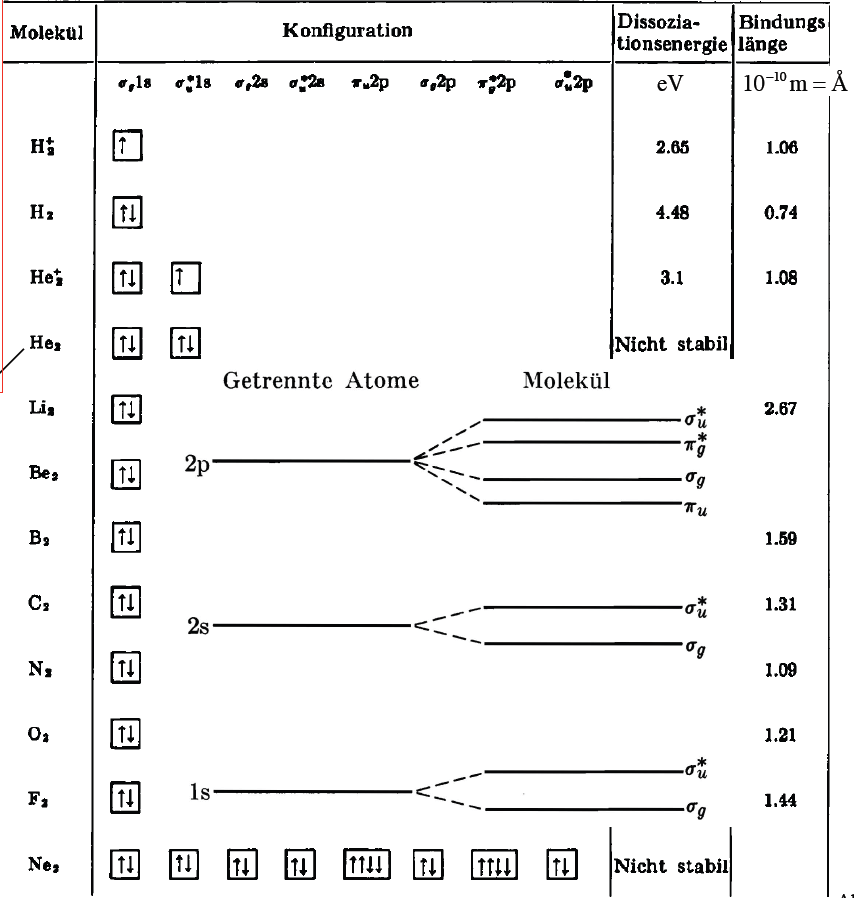
\includegraphics[width = 15cm]{ph_elektronenkonfi.png}
\end{tabular}
\subsection{Hybrid-Wellenfunktionen}
\begin{tabular}{p{4cm} p{15cm}}
 sp	& \\
$sp^2$	& planar-trigonal\\
$sp^3$	& tetraedrisch $(CH_4)$\\
	& \begin{tabular}[t]{ll}
	  $\Psi_1 = \tfrac{1}{2} (s + p_x + p_y + p_z)$	& $\Psi_2 = \tfrac{1}{2} (s + p_x - p_y - p_z)$\\
	  $\Psi_3 = \tfrac{1}{2} (s - p_x + p_y - p_z)$	& $\Psi_4 = \tfrac{1}{2} (s - p_x - p_y + p_z)$
	  \end{tabular}
\end{tabular}
\subsection{Molekulare Rotation}
\begin{tabular}{p{4cm}p{15cm}}
Rotationsenergie eines 2-atomigen Molek�ls	& $E_r = \frac{L^2}{2I} = \frac{\hbar^2}{2I} l(l+1)\quad I =$ Tr�gheitsmoment\\
Auswahlregel (elektr. Dipolstrahlung)		& $\Delta l = \pm 1 \Rightarrow \Delta E_{l,l-1} = 2lE_1\quad E_1 = \frac{\hbar^2}{2I}$\\
\end{tabular}
\subsection{Molekulare Vibration}
Modelliert durch harmonischen Oszillator.\\
\begin{tabular}{p{4cm}p{15cm}}
Vibrationsenergie	& $E_n = \left(n+\frac{1}{2}\right) \hbar\omega$\\
\multicolumn{2}{l}{Pro Vibrationsenergieniveau gibt es also mehrere ($n-1$ viele) Rotationsenergieniveaus.}
\end{tabular}
%Festk�rper
\section{Festk�rper}
kristalline Festk�rper sind in Kristallgitter angeordnet. Davon gibt es einige Formen:\\
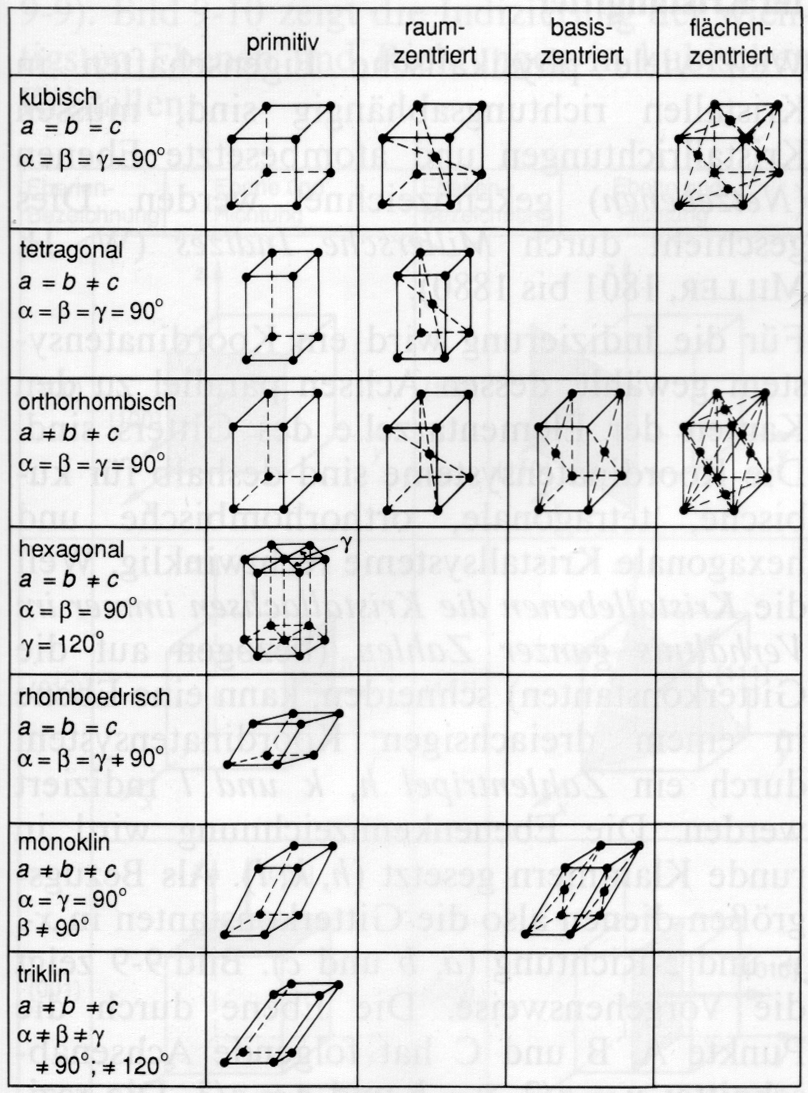
\includegraphics[width = 15cm]{ph_kristallgitter.png}\\
\subsection{Arten von Festk�rper}
\begin{tabular}{p{4cm} p{15cm}}
Kovalente Festk�rper	& \begin{itemize}
                    	  	\item kovalente Bindung: lokalisierte, gerichtete Bindung
				\item starke Bindung: Kristallschwingungen haben eine hohe Frequenz
				\item schlechte Leitf�higkeit: keine freien Elektronen
				\item Beispiele: GaAs, Diamant (beide $sp^3$-Hybridwellenfkt., beide (durchschnittlich) 4 Valenzelektronen.
                    	  \end{itemize}\\
Ionenkristalle		& \begin{itemize}
              		  	\item regelm�ssige Anordnung von positiven und negativen Ionen
				\item Ionen sind so angeordnet, so dass die gegenseitige elektrische WW eine stabile Konfiguration ergibt.
				\item Ionenbindungskraft $<$ kovalente Bindungskraft
				\item Ionen im Kristall angeordnet wie dichtgepackte Kugel.
				\item Beispiele: NaCl
              		  \end{itemize}\\
Molekulare Festk�rper	& \begin{itemize}
                     	  	\item van der Waals-Kr�fte: entsprechen Kr�ften zwischen zwei elektr. Dipolen
				\item Kr�fte aufgrund von instantanen elektrischen Dipolen
                     	  \end{itemize}\\
Metalle			& \begin{itemize}
       			  	\item Elemente mit relativ geringer Ionisationsenergie
				\item Bindung der positiven Ionen durch Elektronengas
				\item Elektronengas: Elektronen bewegen sich frei durch das Kristallgitter und sind nicht lokalisiert.
				\item sehr gute thermische und elektrische Leitf�higkeit
       			  \end{itemize}
\end{tabular}
\subsection{N-atomiges Molek�l}
\begin{tabular}{p{4cm}p{15cm}}
LCAO-Ansatz	& $\Psi(x) = \sum_{n=1}^N \psi(x-na)e^{ikna}$ F�r $N=2$ haben wir die LCAO eines zweiatomigen Molek�ls, z.B. $H_2^+$\\
resultierende Wfkt.	& 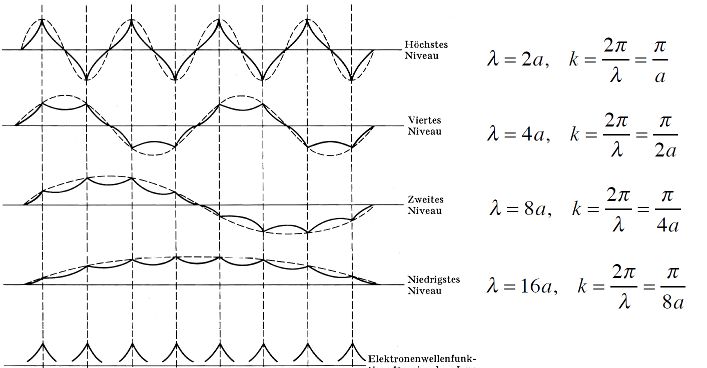
\includegraphics[width=14cm]{ph_n_molecule_lcao_wavefn.png}\\
Wellenzahl	& $k = \frac{n\pi}{Na}\quad n=1,2,...,N$\\
Energieb�nder	& Je gr�sser $n$, desto kleiner werden die Unterschiede zwischen den einzelnen Energiekurven, wodurch sich ein kontinuierliches Energieband ergibt. In einem Kristallgitter kann es mehrere Energieb�nder geben, die jeweils einem der Energieniveaus der Atome entsprechen, die das Gitter bilden.\\
Energie im Band = Breite des Bands	& $E = \frac{p^2}{2m_e} = \frac{\hbar^2k^2}{2m_e}$\\
\end{tabular}
\subsection{Modell freier Elektronen}
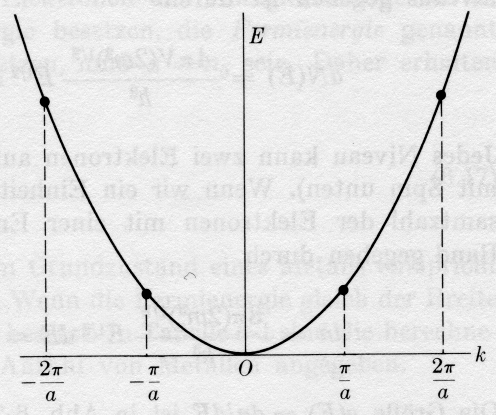
\includegraphics[width = 6cm]{ph_model_free_electrons.png}
\begin{tabular}[b]{p{4cm}p{9cm}}
Wellenfunktion	& $\Psi(x) = e^{ikx}$\\
Impuls		& $p = \hbar k$\\
Energie		& $E = \frac{\hbar k^2}{2m} \propto k^2$\\
Wellenzahl	& $k_{max} = \frac{\pi}{a}$\\
Energie im Band	& $E_{max} = \frac{\hbar^2\pi^2}{2m_ea^2}$\\
Gruppengeschw. Elektronen	& $v_g = \frac{d\omega}{dk} = \frac{1}{\hbar}\frac{dE}{dk},\quad E = \hbar\omega$\\
Kraft		& $F = ma = m\frac{dv_g}{dt}$
\end{tabular}
\subsection{Elektronen in periodischer Struktur}
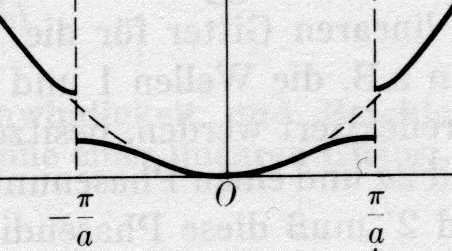
\includegraphics[width = 6cm]{ph_electrons_in_periodic_potential.png}
\begin{tabular}[b]{p{4cm}p{9cm}}
Wellenfunktion (Blochzustand)	& \begin{tabular}[t]{l}
				    $\Psi(x) = e^{ikx}u(x),\quad \underbrace{u(x+a) = u(x)}_{\text{Blochzustand}}$\\
				    $\Psi(x) = \sum_{n=1}^N \psi(x-na)e^{ikna}$ ist ein Blochzustand.
				  \end{tabular}\\
Energie		& Mit der N�herung des tight binding models ergibt sich: $E(k) = E_0 - 2A\cos(k_i a),\quad k_i = \frac{2\pi}{aN}i$\\
effektive Masse	& $\frac{1}{m^{\ast}} = \frac{1}{\hbar^2}\frac{d^2E}{dk^2}$\\
Kraft		& $F = m^{\ast}a = m^{\ast}\frac{dv_g}{dt}$
\end{tabular}
\subsection{Elektronenleitung}
\begin{tabular}{p{4cm}p{15cm}}
Fermienergie $E_F$	& 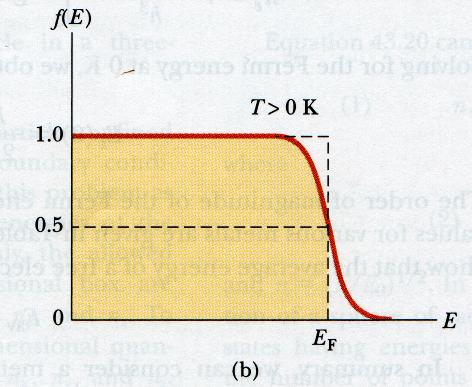
\includegraphics[width = 6cm]{ph_fd_statistics.png}\\
Theorie zur Elektronenleitung	& 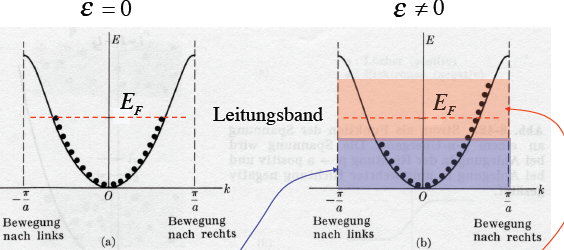
\includegraphics[width = 13cm]{ph_electron_conduction.png}\\
				& blau: gleich viele Elektronen mit Impuls $+p (\propto k)$ wie mit $-p \Rightarrow$ im Mittel Impuls = 0 $\Rightarrow$ kein Strom. Nur Elektronen im roten Bereich tragen zum Strom bei. In vollst�ndig gef�llten B�ndern kann die Verschiebung (Bild links zu Bild rechts) jedoch nicht geschehen. Deshalb keine Leitung\\
Isolator		& Das oberste Band ist vollst�ndig besetzt (Valenzband). Die Energiel�cke zum Leitungsband ist zu hoch. Laut Fermi-Dirac Statistik ist dann die WSK 0, im Leitungsband ein Teilchen zu finden.\\
Metalle			& Das oberste Band ist nicht voll. Die Fermienergie liegt im Leitungsband.\\
Halbleiter		&  Es gibt zwar ein Valenzband, doch die Energiel�cke zum n�chsth�heren Band (Leitungsband) ist klein genug, sodass es eine WSK gibt, ein Teilchen im Leitungsband zu finden.
\end{tabular}
\subsection{Zustandsdichte}
Die Zustandsdichte gibt an, wie viele Zust�nde pro $k$ oder $E$ existieren. Man macht dazu zwei Annahmen:
\begin{enumerate}
	\item Kristallw�rfel der Kantenl�nge $L$ mit unendliche hohen Potentialbarrieren am Rand des W�rfels. $\Psi($Rand des W�rfels$) = 0$
	\item Periodische Randbedingungen $\Psi(x,y,z) = \Psi(x+L,y+L,z+L)$
\end{enumerate}
\subsubsection{Zustandsdichte im $\vec{k}$-Raum}
Da wir in 3D sind, brauchen wir den Vektor $\vec{k}$ und nicht nur den Skalar $|\vec{k}|$\\
\begin{tabular}{p{4cm}p{15cm}}
Wellenfkt. 1D-Potentialtopf	& $\Psi_n(x,t) = \sqrt{\frac{2}{L}} \sin\frac{n\pi x}{L}\exp\left(-i\frac{E_n}{\hbar}t\right)\quad k_n = \pm\frac{n\pi}{L}$ (pro $n$ \textbf{zwei} $k_n$ !)\\
Volumen eines Zustands		& \begin{tabular}[t]{llll}
				  1D	& $(\Delta k) \cdot 2 \cdot 1$		&						& $ = \left(\frac{2\pi}{L}\right)$\\
				  2D	& $(\Delta k)^2 \cdot 2 \cdot 2$	& $ = \left(\frac{\pi}{L}\right)^3 \cdot 4$	& $ = \left(\frac{2\pi}{L}\right)^2$\\
				  3D	& $(\Delta k)^3 \cdot 2 \cdot 3$	& $= \left(\frac{\pi}{L}\right)^3 \cdot 8$	& $ = \left(\frac{2\pi}{L}\right)^3$\\
				  \end{tabular}
				  $\Delta k = \frac{\pi}{L}$\\
Zustandsdichte			& \begin{tabular}[t]{lll}
				  \multicolumn{3}{p{14cm}}{Pro (r�umlichen) Zustand gibt es 2 Elektronen (Spin up, Spin down). Das Volumen eines solchen Zustands ist oben angegeben. F�r die Zustandsdichte gilt also allgemein $D = \frac{2}{\text{Zustandsvolumen}}$}\\
				  1D							& 2D							& 3D\\
				  $D_1(k) = \frac{2}{\left(\frac{2\pi}{L}\right)}$	& $D_2(k) = \frac{2}{\left(\frac{2\pi}{L}\right)^2}$	& $D_3(k) = \frac{2}{\left(\frac{2\pi}{L}\right)^3}$
				  \end{tabular}
\end{tabular}
\subsubsection{Zustandsdichte im $E$-Raum}
Die Zustandsdichten aus dem $\vec{k}$-Raum m�chten wir nun in den $E$-Raum �bersetzen. Daf�r m�ssen wir aber von $\vec{k}$ nach $|\vec{k}|$ kommen.\\
\begin{tabular}{p{4cm}p{15cm}}
Zustandsdichten im $|\vec{k}|$-Raum	& \begin{tabular}[t]{lll}
 				  \multicolumn{3}{p{14cm}}{F�r die Zustandsdichte gilt allgemein $D = \frac{\text{Volumen mit konstantem $\vec{k}$}}{\text{Zustandsvolumen}}\cdot 2$}\\
				  1D								& 2D							& 3D\\
				  $D_1(k) = \frac{dk}{\left(\frac{2\pi}{L}\right)}\cdot 2$	& $D_2(k) = \frac{2\pi k dk}{\left(\frac{2\pi}{L}\right)^2}\cdot 2$	& $D_3(k) = \frac{4\pi k^2 dk}{\left(\frac{2\pi}{L}\right)^3}\cdot 2$
				  \end{tabular}\\
Beziehung $E$-$|\vec{k}|$ (Modell freier Elektronen)	& \begin{tabular}[t]{l}
				    $E = \frac{\hbar^2 k^2}{2m_e} \Leftrightarrow k = \sqrt{\frac{2m_e E}{\hbar^2}}$\\
				    $\frac{dk}{dE} = \sqrt{\frac{2m_e}{\hbar^2}}\frac{1}{2\sqrt{E}}$
				  \end{tabular}\\
Zustandsdichten im $E$-Raum	& \begin{tabular}[t]{|l|l|l|}
				  \hline
				  $D_1(E) = \frac{L}{\pi\hbar}\sqrt{\frac{2m_e}{E}} dE$	& $D_2(E) = \frac{L^2m_e}{\pi\hbar^2} dE$	& $D_3(E) = \frac{L^3}{2\pi^2}\left( \frac{2m_e}{\hbar^2} \right)^{\frac{3}{2}} \sqrt{E} dE$\\\hline
				  \end{tabular}\\
Zusammenh�nge			& \begin{tabular}[t]{l}
				    $g(E) = \frac{D(E)}{V}$\\
				    $D(E) = \frac{dN}{dE}\quad $ N: Total Anzahl Elektronen in V\\
				    $g(E) = \frac{dn}{dE}\quad $ n: Elektronendichte\\
				    $n = \int_0^{E_F}g(E) dE$
				  \end{tabular}
\end{tabular}
\subsubsection{Alternative Herleitung f�r $D_3$}
\begin{tabular}[t]{p{4cm}p{15cm}}
Anzahl Energiezust�nde in einem 3D Kasten	& \begin{tabular}[t]{l}
							    $\tilde{N}(E) = \boldsymbol{\tfrac{1}{8} \pi k^3} = \frac{8\pi V}{3h^3} (2m^3)^{\frac{1}{2}} E^{\frac{3}{2}}\quad V:$ Volumen des Kastens\\
							    $\tilde{D}_3(E) := \frac{d\tilde{N}}{dE} = \frac{4\pi V (2m^3)^{\frac{1}{2}}}{h^3}E^{\frac{1}{2}} = \frac{L^3}{2\pi^2}\left( \frac{2m_e}{\hbar^2} \right)^{\frac{3}{2}} \sqrt{E} dE$\\
							  \end{tabular}\\
Gesamtzahl der Elektronen innerhalb $E + dE$	& \begin{tabular}[t]{p{14cm}}
						   Jeder Energiezustand kann zwei Elektronen aufnehmen (Spin up, down). Also $d\tilde{N}$ mit 2 multiplizieren.\\
						   $D_3(E) := \frac{d\tilde{N}}{dE} = \frac{8\pi V (2m^3)^{\frac{1}{2}}}{h^3}E^{\frac{1}{2}}$
						  \end{tabular}\\
\end{tabular}
\subsection{L�cher}
Als L�cher bezeichnet man fehlende Elektronen im Valenzband. L�cher sind also nur Gedankenkonstrukte, die das Rechnen vereinfachen. Sie haben folgende Eigenschaften:\\
\begin{tabular}{ll}
Ladung: +e				& Impuls: $k_h = -k_e$\\
Energie: $E_h(k_h) = -E_e(k_e)$		& effektive Masse: $m_h^{\ast} = -m_e^{\ast}$
\end{tabular}\\
\begin{tabular}{p{4cm}p{15cm}}
Fermi-Dirac WSK-Verteilung		& $f(E) = \frac{1}{e^{(E-E_F)/k_BT}+1}$\\
Elektronendichte im Leitungsband	& $n = \int_{E_L}^{\infty} f(E)g(E)dE \quad g(E) = \frac{8\pi \sqrt{2(m_e^{\ast})^3}}{h^3}\sqrt{E-\boldsymbol{E_L}}$\\
					& Resultat: $\boxed{n = N_C \exp\left(-\frac{E_L-E_F}{k_BT}\right), \quad N_C \equiv 2 \left( \frac{2\pi m_e^{\ast}k_BT}{h^2} \right)^{\frac{3}{2}}}$\\
L�cherdichte im Valenzband		& $p = \int_{0}^{E_V} (1-f(E))g(E)dE \quad g(E) = \frac{8\pi \sqrt{2(m_{hole}^{\ast})^3}}{h^3}\sqrt{\boldsymbol{E_V}-E}$\\
					& Resultat: $\boxed{p = N_V \exp \left( -\frac{E_F-E_V}{k_BT} \right), \quad N_V \equiv 2 \left(\frac{2\pi m_{hole}^{\ast}k_BT}{h^2} \right)^{\frac{3}{2}}}$\\
Fermienergie eines intrinsischen Halbleiters (ohne Fremdatome, $\Rightarrow n = p$)	& $E_F \equiv E_i = \frac{E_L + E_V}{2} + \frac{k_BT}{2}\ln\left(\frac{N_V}{N_C}\right)$\\
Ladungstr�gerdichte eines intri. Halbleiters	& $n_i = \sqrt{n\cdot p} = \sqrt{N_LN_V}\exp \left( -\frac{E_g}{2k_BT} \right)\quad E_g \equiv E_L-E_V$ Bandgap energy (Bsp: GaAs 1.43eV)\\
Stromdichte				& $j = nqv$\\
					& \begin{tabular}[t]{l}
					    n: Zahl der Teilchen (z.B. Elektronen) pro Volumeneinheit\\
					    q: Ladung der Teilchen. q = -e = -1.602 $\cdot 10^{-19}A\cdot s$ Elementarladung der Elektronen\\
					    v: Driftgeschwindigkeit der Ladungstr�ger (z.B. Elektronen)
					  \end{tabular}\\
Stromrichtung				& Per Definition: von plus nach minus\\
Kraft des elektrischen Felds		& $F = qE$\\
Driftgeschwindigkeit im Halbleiter	& $v_d = \mu E\quad [\mu] = cm^2V^{-1}s^{-1}:$ Mobilit�t\\
Stromdichte im Halbleiter		& $j = \sigma E\quad \sigma = e\mu_n n + e \mu_p p\quad \mu_p \ll \mu_n$
\end{tabular}
\subsection{Absorption und Emission von Photonen}
\begin{tabular}{p{4cm}p{15cm}}
Absorption	& Absorption eines Photons mit $E = h\nu$ entspricht einem �bergang eines Elektrons vom Valenzband ins Leitungsband. Die Bandl�ckenenergie $E_g$ entspricht $h\nu$\\
Emission	& Emission eines Photons entspricht einem �bergang eines Elektrons vom Leitungsband ins Valenzband.
\end{tabular}
\subsection{Dotierungen}
``St�rstellen'' eines intrinsischen Halbleiters. Dadurch ver�ndert sich die Fermienergie und weitere Parameter gegen�ber einem intrinsischen Halbleiter.\\
\begin{tabular}{p{4cm}p{15cm}}
Donatoren	& Fremdatome, die mehr Elektronen beitragen k�nnen. Bsp: P (5 Aussen$e^-$) in Si(4 Aussen$e^-$) $\Rightarrow$ Das �berz�hlige Elektron liegt auf einem Energielevel knapp unter $E_L$. Es kann also leicht ins Leitungsband angeregt werden, wo es leiten kann.\\
Akzeptor	& Fremdatome, die weniger Elektronen (= mehr L�cher) haben. Bsp: Al (3 Aussen$e^-$) in Si $\Rightarrow$. Das �berz�hlige Loch ist auf einem Energielevel, das knapp �ber $E_V$ liegt. Ein Elektron aus dem Valenzband kann nun das Loch besetzen und somit ein Loch im Valenzband freigeben, das zur Leitung genutzt werden kann.\\
Elektronendichte im Leitungsband	& $n = \frac{N_D^+-N_A^-}{2}+ \sqrt{\left( \frac{N_D^+-N_A^-}{2} \right)^2 + n_i^2},\quad N_D^+ > N_A^-\quad N_D^+:$ Dichte von Donor-Atomen\\
L�cherdichte im Valenzband		& $p = \frac{N_A^--N_D^+}{2}+ \sqrt{\left( \frac{N_A^--N_D^+}{2} \right)^2 + n_i^2},\quad N_A^- > N_D^+\quad N_A^-:$ Dichte von Akzeptor-Atomen\\
Fermienergie im n-dotierten Halbl.	& $E_{F_n} = E_i + k_BT \ln \left(\frac{n}{n_i} \right)$\\
Fermienergie im p-dotierten Halbl.	& $E_{F_p} = E_i - k_BT \ln \left( \frac{p}{n_i} \right)$
\end{tabular}
%Statistische Mechanik
\section{Klassische statistische Mechanik}
\subsection{mikroskopische Bedeutung von Druck und Temperatur}
\begin{tabular}{p{4cm} p{15cm}}
$k_B$	& $k_B = 1.3807 \cdot 10^{-23} J/K$\\
Geschwindigkeit	& \begin{tabular}[t]{l}
               	  $\langle v_x^2 \rangle = \frac{1}{N} \sum_{i=1}^N v_{xi}^2$\\
		  Bewegung isotrop: $\langle v_x^2 \rangle = \langle v_y^2 \rangle = \langle v_z^2 \rangle = \frac{1}{3} \langle v^2 \rangle$\\
		  $\langle v^2 \rangle = \langle v_x^2 \rangle + \langle v_y^2 \rangle + \langle v_z^2 \rangle$
               	  \end{tabular}\\
Druck	& \begin{tabular}[t]{l}
     	   $p = \frac{F}{A}$\\
	   $p = \frac{1}{3} \rho \langle v^2 \rangle$\\
	   $p = \frac{2}{3}\frac{N}{V} \left( \frac{1}{2}m \langle v^2 \rangle \right) = \frac{2}{3} \frac{N}{V} \langle E_{kin} \rangle \Leftrightarrow pV = \frac{2}{3}N\langle E_{kin} \rangle (\ast)$
     	  \end{tabular}\\
Dichte	& $\rho = \frac{mN}{V}$\\
Zustandsgleichung ideales Gas	& $pV = Nk_B T$\\
Temperatur: �quipartitionsgesetz	& Mit der Zustandsgleichung ergibt sich aus $(\ast) \langle E_{kin} \rangle = \frac{3}{2}k_BT$. Isotropie vorausgesetzt, ist die innere Energie also pro Freiheitsgrad $\langle E_{kin,j} \rangle = \frac{1}{2} k_BT\quad j = x,y,z$.\\
			& $\langle E_{kin} = U \rangle = \frac{f}{2} k_BT\quad $ f = \# Freiheitsgrade $\cdot$ \# Molek�le $\quad U:$ Innere Energie\\
G�ltigkeit �PG		& Das �quipartitionsgesetz ist bei tiefen Temperaturen nicht mehr g�ltig, wegen der Quantisierung der Energiezust�nde.\\
Freiheitsgrade		& \begin{tabular}[t]{ll}
			    \multicolumn{2}{l}{F�r zweiatomige Molek�le gelten bspw. folgende Freiheitsgrade}\\
			    Translation des Schwerpunkts	& $f=3$\\
			    Rotation				& $f=2$\\
			    Vibration				& $f=2$
			  \end{tabular}
\end{tabular}\\

\subsection{Ensembles}
\begin{tabular}{p{4cm} p{15cm}}
$n_i$	& Anz. Teilchen\\
$P$	& WSK, dass ein System in einer bestimmten Zustandskonfiguration ist.\\
$g_i$	& WSK, ein Teilchen in einem bestimmtem Zustand zu finden.\\
Thermodyn. Glgw. (TG)	& dP = 0\\
\end{tabular}
\subsubsection{Kanonisches Ensemble}
\begin{tabular}{p{4cm} p{15cm}}
Konstanten	& $N,V,T$\\
Fluktuationen	& $E$\\
		& $N = \sum_i n_i$\\
$g_i$ (unter TG)	& $\boxed{g_i = \frac{1}{Z(N,V,T)} e^{-\beta E_i}}$\\
Kanonische Zustandssumme	& $\boxed{Z(N,V,T) = \sum_i g_i e^{-\beta E_i}}\quad \beta = \frac{1}{k_BT}$\\
Energie				& $\boxed{\langle E \rangle = \sum_i g_i E_i} = - \left( \frac{\partial \ln Z(N,V,T)}{\partial \beta} \right)_{N,V}$\\
Druck			& $\langle p \rangle = \frac{1}{\beta} \left( \frac{\partial \ln Z(N,V,T)}{\partial V} \right)_{N,\beta}\quad \Delta E_i = -p_i\Delta V$\\
Entropie		& $S = -k_B \sum_i g_i \ln g_i$\\
Zustandssumme ideales Gas	& \begin{tabular}[t]{l}
				      $Z_{id} = \sum_i g_i e^{-E_i/k_BT} = \int_0^{\infty} D_3(E) e^{-E/k_BT} dE$\\
				      $\quad D_3(E) = \frac{L^3}{2\pi^2}\left( \frac{2m}{\hbar^2} \right)^{\frac{3}{2}} \sqrt{E} dE$\\
				      $Z_{id} = \frac{V(2\pi mk_BT)^{3/2}}{h^3} = V\left( \frac{m}{2\beta\pi\hbar^2} \right)^{\tfrac{3}{2}}$
				  \end{tabular}\\
Anzahl Molek�le w.r.t. Energie	& $dn = \frac{N}{Z}e^{-E/k_BT}D(E) dE$\\
				& 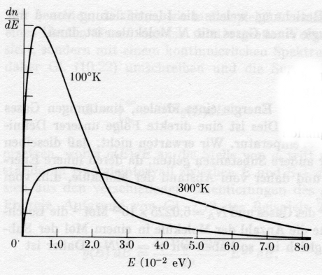
\includegraphics[width = 7cm]{ph_statmech_dndE.png} 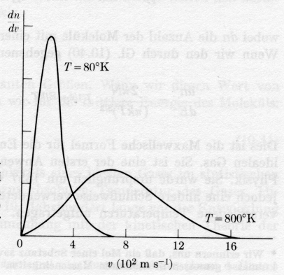
\includegraphics[width = 7cm]{ph_statmech_dndv.png}\\
\end{tabular}
\subsubsection{Maxwell-Boltzmann-Verteilung}
\begin{tabular}{p{4cm} p{15cm}}
Zustandssumme		& $Z(N,V,T) = \frac{1}{N!}[z(V,T)]^N$\\
Ideal Gas		& \\
Avg. size of velocity	& $\langle v \rangle = \sqrt{ \frac{8k_BT}{m\pi} }$\\
Root mean square	& $\langle v^2 \rangle^\frac{1}{2} = \sqrt{ \frac{3k_BT}{m} }$\\
most probable speed	& $v_{mp} = \sqrt{ \frac{2k_BT}{m}}$\\
Avg. kinetic energy	& $\langle E \rangle = N \frac{3}{2} k_BT$\\
Heat capacity		& $\frac{dE}{dT} = \frac{3}{2} Nk_B$\\
Free energy		& $F = -Nk_BT \left( \frac{3}{2} \ln \left(\frac{2\pi mk_BT}{h^2} \right) - \ln \left( \frac{N}{V} \right) + 1 \right)$\\
Entropy			& $S = Nk_B \left( \frac{3}{2} \ln \left(\frac{2\pi mk_BT}{\hbar^2} \right) - \ln \left( \frac{N}{V} \right) + \frac{5}{2} \right)$
\end{tabular}
\subsection{Fermi-Dirac, Bose-Einstein partition functions}
\begin{tabular}{p{4cm} >{$}p{16cm}<{$}}
System			& \text{
			    \begin{tabular}{l}
			      Volume: $V$\\
			      Number of particles: $N$\\
			      Energy levels: $E_j$\\
			      1-particle energy levels: $\epsilon_k$\\
			      Number of particles in a quantum state $\Psi_k: m_k$\\
			    \end{tabular}
			  }\\
			& E_j = \sum_k m_k\epsilon_k; N = \sum_k m_k\\
Grand-canonical partition function	& Z(\mu,V,T) = \sum_{N=0}^{\infty}\sum_j e^{-\beta (E_j-\mu N)} = ... = \prod_k\sum_{m_k} \left( e^{-\beta(\epsilon_k-\mu)}\right)^{m_k}\\
Fermi-Dirac partition function	& m_k = 0 \vee 1 \Rightarrow Z_{FD} (\mu,V,T) = \prod_k \left[ 1+e^{-\beta(\epsilon_k-\mu)} \right]\\
Bose-Einstein partition function	& m_k = 0,1,2,... \Rightarrow Z_{BE} (\mu,V,T) = \prod_k \left[ 1-e^{-\beta(\epsilon_k-\mu)} \right]^{-1}\\
Combined partition function		& Z_{FD/BE}(\mu,V,T) = \prod_k \left[ 1\pm e^{-\beta(\epsilon_k-\mu)} \right]^{\pm 1}
\end{tabular}\\
\subsection{Fermi-Dirac Statistics}
\begin{tabular}{p{4cm} >{$}p{16cm}<{$}}
Avg. Number of particles	& \langle N \rangle = \frac{1}{\beta} \left( \frac{\partial \ln Z_{FD}(\mu,V,T) }{\partial \mu} \right)_{V,T} = ... = \sum_k \left(e^{+\beta(\epsilon_k-\mu)} + 1 \right)^{-1} = \sum_k \langle m_k \rangle\\
$\langle m_k \rangle$		& \langle m_k \rangle = e^{-\beta(\epsilon_k-\mu)}\quad \langle m_k \rangle << 1 \text{ (Boltzmann Limit) }\\
Avg. Energy			& \langle E \rangle = \sum_k \langle m_k \rangle \epsilon_k = \sum_k \frac{\epsilon_k}{e^{+\beta(\epsilon_k-\mu)} + 1}\\
Pressure			& pV = k_BT\ln Z_{FD}(\mu,V,T) = k_BT \sum_k \ln \left( 1 + e^{-(\epsilon_k-\mu)/k_BT} \right)
\end{tabular}
\subsection{Bose-Einstein Statistics}
\begin{tabular}{p{4cm} >{$}p{16cm}<{$}}
Avg. Number of particles	& \langle N \rangle = \frac{1}{\beta} \left( \frac{\partial \ln Z_{BE}(\mu,V,T) }{\partial \mu} \right)_{V,T} = ... = \sum_k \left(e^{+\beta(\epsilon_k-\mu)} - 1 \right)^{-1} = \sum_k \langle m_k \rangle\\
$\langle m_k \rangle$		& \langle m_k \rangle = e^{-\beta(\epsilon_k-\mu)}\\
Avg. Energy			& \langle E \rangle = \sum_k \langle m_k \rangle \epsilon_k = \sum_k \frac{\epsilon_k}{e^{+\beta(\epsilon_k-\mu)} - 1}\\
Pressure			& pV = k_BT\ln Z_{BE}(\mu,V,T) = -k_BT \sum_k \ln \left( 1 - e^{-(\epsilon_k-\mu)/k_BT} \right)
\end{tabular}


%Thermodynamik
\section{Thermodynamik}
\begin{tabular}{p{4cm} p{15cm}}
Spezifische Gr�ssen	& $x = \frac{X}{m}$ \begin{tabular}{|ll}
                  	                         x:	& spezifische Zustandsgr�sse\\
						 X:	& Zustandsgr�sse\\
						 m:	& Masse $[kg]$
                  	                        \end{tabular}\\
Molare Gr�ssen	& $X_m = \frac{X}{m}M$ \begin{tabular}{|ll}
                  	                         $X_m$:	& molare Zustandsgr�sse\\
						 X:	& Zustandsgr�sse\\
						 M:	& Molmasse $[kg/mol]$
                  	                        \end{tabular}\\
Masse vs. molare Masse	& $m = n\cdot M$\\
Konstanten	& \begin{tabular}[t]{ll}
          	   universelle Gaskonstante	& $R = 8.314 \frac{J}{mol K}$\\
		   Avogadro-Konstante		& $N_A = 6.022 \cdot 10^{23} \frac{1}{mol}$\\
		   Boltzmann-Konstante		& $k_B = \frac{R}{N_A} = 1.38 \cdot 10^{-23}\frac{J}{K}$\\
						& $k_BT|_{T=300K} = 25.8 meV$
		  \end{tabular}\\
Molmasse etc.	& \begin{tabular}[t]{ll}
		   Molmasse einer Substanz A	& $M = N_Am_A$\\
		   Atom- oder Molek�lmasse einer Substanz A	& $m_A$\\
		   Total Anzahl Molek�le	& $N$\\
		   Anzahl Mole einer Substanz	& $n$\\
          	  \end{tabular}\\
Kelvin-Celsius	& $T[K] = \vartheta[^\circ C] + 273.15$\\
Zustandsgleichung ideales Gas	& $\boxed{pV = nRT = \frac{N}{N_A}RT = Nk_BT}$\\
Thermische Ausdehnung	& \begin{tabular}[t]{ll}
                     	   Festk�rper	& 1D: $\frac{\Delta l}{l} = \alpha \Delta T$\\
					& 3D: $\frac{\Delta V}{V} = \gamma \Delta T$ Isotrop $\Rightarrow \gamma = 3\alpha\quad\gamma\approx 10^{-5}K^{-1}$\\
			   Fl�ssigkeiten	& $\frac{\Delta V}{V} = \gamma\Delta T \quad\gamma\approx 10^{-3}K^{-1}$\\
						& $\rho = \frac{m}{V} = \frac{m}{V_0(1+\gamma\Delta T)} \approx \rho_0(1-\gamma\Delta T)$
                     	  \end{tabular}\\
\end{tabular}
\subsection{1.Hauptsatz (Energieerhaltung)}
\begin{tabular}{p{4cm} p{15cm}}
\textbf{1.Hauptsatz}	& $\boxed{dU = \partial Q + \partial W}\quad [Q] = J, [T] = K$\\
		& $U$: innere Energie, $W$: Arbeit, $Q$: W�rme. $U$ ist eine Zustandsgr�sse, w�hrend $W$ und $Q$ vom Weg abh�ngen (deshalb das $\partial$-Zeichen).\\
�quipartitionsgesetz ideales Gas	& $U = N\cdot \frac{f}{2} k_BT$\\
\textbf{W�rme} $Q$	& $\boxed{\partial Q = CdT}\quad C$: W�rmekapazit�t des Systems $\quad [C] = \frac{J}{K}$\\
			& W�rme ist eine Energie aufgrund von Temperaturunterschieden. Die Energie�bertragung ist dabei irreversibel.\\
spezifische W�rmekapazit�t	& $c = \frac{C}{m}\quad [c] = \frac{J}{kg\cdot K}$\\
molare W�rmekapazit�t		& $C_m = M\cdot c \quad[C_m] = \frac{J}{mol\cdot K}$\\
elektr. W�rme�quivalent		& $cm\Delta T = Q = W_{el} = VI\Delta t\quad V:$ Spannung, $I:$ Stromst�rke\\
isobare W�rmekapazit�t	& $C_p = \left(\frac{\partial Q}{dT} \right)_p$\\
isochore W�rmekapazit�t	& $C_V = \left(\frac{\partial Q}{dT} \right)_V$\\
F�r ideales Gas	& \begin{tabular}[t]{|l}
               	  $C_{mp} = C_{mV} + R\quad C_{mX}$: molare W�rmekapazit�t bei konstantem X\\
		  $C_{mp} = \left(\frac{f}{2} + 1 \right) R,\quad C_{mv} = \frac{f}{2} R,\quad R =$ Gaskonstante\\
		  $\kappa = \frac{C_{mp}}{C_{mV}} = 1 + \frac{2}{f}$
               	  \end{tabular}\\
Erwartungswert der Energie eines harm.Osz.	& $\langle E \rangle = \sum_{n=0}^{\infty}W_nE_n = \frac{1}{2}\hbar\omega + \frac{\hbar\omega}{e^{\hbar\omega/k_BT}-1}, \quad W_n = \frac{e^{-E_n/k_BT}}{\sum_n e^{-E_n/k_BT}}$\\
F�r kristalline Festk�rper	& \begin{tabular}[t]{l}
                          	   $U_{osz} = 3N\langle E \rangle = 3N\left(\frac{1}{2} \hbar \omega + \frac{\hbar \omega}{e^{\hbar\omega/k_BT}-1} \right)$\\
				   $C_V = \left(\frac{\partial Q}{dT}\right)_V \xrightarrow{dU = \partial Q-pdV}= \frac{dU_{osz}}{dT} = 3N\frac{d}{dT}\langle E \rangle$\\
				   $C_V = 3Nk_B \left[ \left( \frac{\hbar\omega}{k_BT} \right)^2 \frac{e^{\hbar\omega/k_BT}}{(e^{\hbar/k_BT}-1)^2} \right]\quad$ Einsteinmodell
                          	  \end{tabular}\\
\textbf{Arbeit} $W$	& $\boxed{\partial W = -pdV}$\\
			& $W_{12} = \int_{V1}^{V2} pAds = \int_{V1}^{V2} pdV$
\end{tabular}
\subsubsection{Zustands�nderungen (Spezialf�lle der Zustandsgleichung)}
Zustandsgleichung ideales Gas: $pV = nRT = Nk_BT$\\
\begin{tabular}{m{1cm}p{2cm}p{3cm}p{3cm}p{4cm}p{4cm}}
				& Bedingung	& thermische Zustandsgr�ssen	& erster Hauptsatz	& W�rme		& Volumen�nderungsarbeit\\\midrule
\rotatebox{90}{isotherm}	& $dT = 0$ \newline $T$ = konst.	& $pV =$ konst.			& $\partial Q + \partial W = 0$ \newline $Q_{12} + W_{12} = 0$	& $\partial Q = -\partial W$ \newline $Q_{12} = nRT \ln \frac{V_2}{V_1}$		& $\partial W = -p dV$ \newline $W_{12} = nRT\ln\frac{V_1}{V_2}$\\\midrule
\rotatebox{90}{isochor}		& $dV = 0$ \newline $V$ = konst.	& $\frac{p}{T} =$ konst. 	& $dU = \partial Q$ \newline $U_2-U_1 = Q_{12}$					& $\partial Q = nC_{mV} dT$ \newline $Q_{12} = nC_{mV}(T_2-T_1)$				& $\partial W = 0$ \newline $W_{12} = 0$\\\midrule
\rotatebox{90}{isobar}		& $dp = 0$ \newline $p$ = konst.	& $\frac{V}{T} =$ konst. 	& $dU = \partial Q + \partial W$ \newline $U_2-U_1 = \newline Q_{12} + W_{12}$		& $\partial Q = nC_{mp}dT$ \newline $Q_{12} = nC_{mp}(T_2-T_1)$		& $\partial W = p dV$ \newline $W_{12} = p(V_1-V_2)$\\\midrule
\rotatebox{90}{isentrop (Adiabate)}	& $dS = 0$ \newline $\partial Q = 0$ \newline $S$ = konst.	& $pV^{\kappa} =$ konst. \newline $TV^{\kappa -1} = $konst. \newline $p^{1-\kappa}T^{\kappa}$ = konst.	& $dU = \partial W$ \newline $U_2-U_1 = W_{12}$		& $\partial Q = 0$ \newline $Q_{12} = 0$		& $\partial W = nC_{mV} dT$ \newline $W_{12} = nC_{mV}(T_2-T_1) \newline = \frac{p_2V_2 - p_1V_1}{\kappa -1}$\\\midrule
\end{tabular}\\
\\ Merke: $\boxed{nC_{mV} = mC_V\qquad
1 $l$ = 1 $dm$^3$ = $10^{-3} $m$^3}$
\subsection{2.Hauptsatz}
\begin{tabular}{p{4cm} p{15cm}}
Entropie $S$	& $S = k_B \ln P$\\
Prozesse	& \begin{tabular}[t]{ll}
        	   $dS > 0$	& irreversibel\\
		   $dS = 0$	& reversibel
        	  \end{tabular}\\
reversibel	& System zu jedem Zeitpunkt im statistischen Gleichgewicht, also $dP = 0$ (most probable distribution)\\
		& F�r reversible Prozesse gilt: $dS = \frac{\partial Q}{T} \Leftrightarrow \boxed{Q = \oint TdS}$
\end{tabular}
\subsubsection{Entropie f�r Maxwell-Boltzmann-Statistik}
\begin{tabular}{p{4cm}p{15cm}}
$\ln P$		& $\ln P ~\propto~ \sum_i n_i\ln g_i - \sum_i \ln (n_i!)$\\
		& $\ln P \approx N- \sum_i n_i \ln \frac{n_i}{g_i}\quad$, wobei $\ln(x!) = x\ln x -x$\\
Entropie f�r Maxwell-Boltzmann-Statistik & \begin{tabular}[t]{l}
                                            $S = k_B \ln P = k_BN - k_B \sum_i n_i \ln \frac{n_i}{g_i}$\\
					    $\qquad$ Aus M-B-Stat bekannt: $\frac{n_i}{g_i} = \frac{N}{Z} e^{-E_i/k_BT}$\\
					    $\Rightarrow S = k_BN + \sum_i n_i \left(\frac{E_i}{T} + k_B \ln \frac{Z}{N} \right)$\\
					    $\qquad N = \sum_i n_i, U = \sum_i n_iE_i$\\
					    $\boxed{S = k_BN + \frac{U}{T} + k_BN \ln \frac{Z}{N}}$
                                           \end{tabular}\\
innere Energie	& $dU = \underbrace{\sum_i E_i dn_i}_{\partial Q} + \underbrace{\sum_i n_idE_i}_{\partial W}$\\
Beispiel ideales Gas	& \begin{tabular}[t]{l}
			    $Z = \frac{V(2\pi mk_BT)^{\frac{3}{2}}}{h^3}$\\
			    $U = \frac{3}{2} k_BNT$\\
			    $\Rightarrow S = k_BN + k_BN \ln \left(\frac{V(2\pi mk_BT)^{\frac{3}{2}}}{h^3N}\right)$
			  \end{tabular}\\
Beispiel irreversibler Prozess	& \begin{tabular}[t]{l}
				   Isotherme ($T$ = konst.) Expansion eines idealen Gases ($N$ = konst.)\\
				   $\Delta S = S_2 - S_1 = k_BN \ln \frac{V_2}{V_1} > 0$\\
				  \end{tabular}
\end{tabular}
\subsubsection{Kreisprozesse}
\begin{tabular}{p{4cm} p{15cm}}
Kreisprozess	& 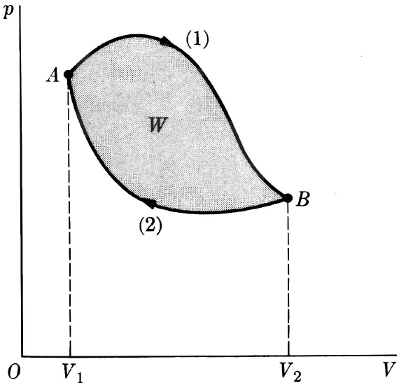
\includegraphics[width = 7cm]{ph_kreisprozess.png}\\
Arbeit		& $W_{Kreis} = \oint pdV\quad$ Fl�che unter (1) - Fl�che unter (2)\\
Wirkungsgrad	& $\eta = \frac{\text{Nutzen (abgegebene W�rme)}}{\text{Aufwand (zugef�hrte W�rme)}} = \frac{|W|}{Q_{zu}}$\\
Leistung	& $P = \frac{\text{Arbeit}}{\text{Zeit}}$
\end{tabular}
\subsubsection{Carnot-Prozess}
\begin{tabular}{p{4cm}p{15cm}}
Prinzip		& \begin{tabular}[t]{p{6cm}p{8cm}}
		    \multicolumn{2}{p{14cm}}{theoretischer, reversibler und optimaler (bzgl. Wirkungsgrad) Kreisprozess mit 2 Isotherme und 2 Isentrope}\\
		    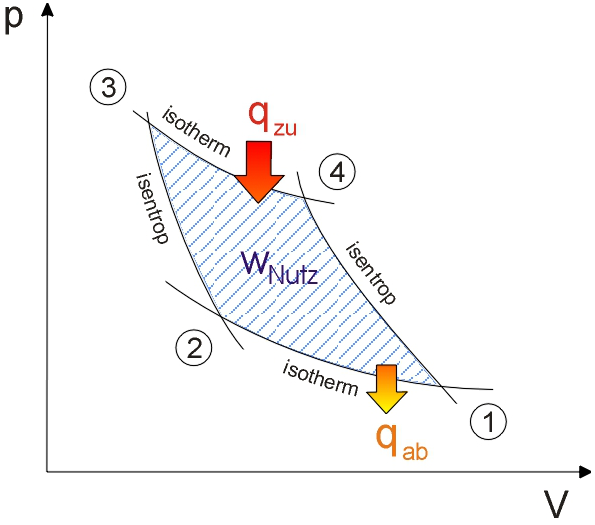
\includegraphics[width = 7.5cm]{ph_carnotprozess_pV.png}	& 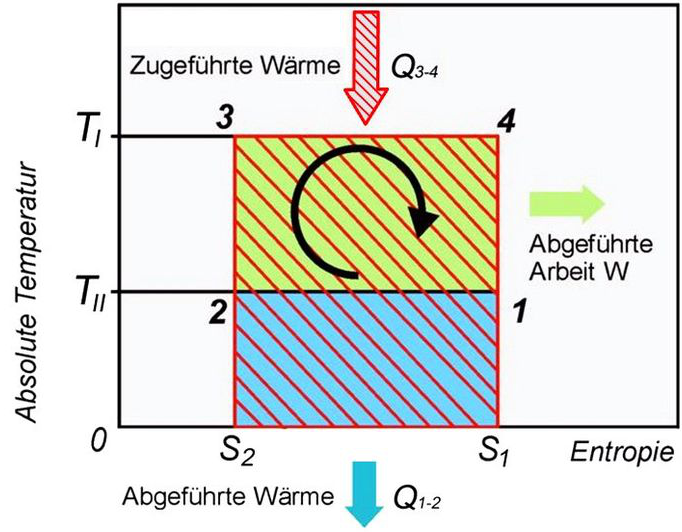
\includegraphics[width = 7.5cm]{ph_carnotprozess_TS.png}\\
		    \multicolumn{2}{l}{1 $\rightarrow$ 2: isotherme Kompression (Gas mit W�rmebad der Temperatur $T_1$ verbunden)}\\
		    $W_{12} = nRT_1 \ln \frac{V_1}{V_2} > 0$	& $Q_{12} = \int_{S_1}^{S_2}TdS = T_3(S_2-S_1) < 0 = -W_{12} $\\\midrule
		    \multicolumn{2}{l}{2 $\rightarrow$ 3: isentrope Kompression (Gas wird vom W�rmebad getrennt)}\\
		    $W_{23} = nC_{mV}(T_3 - T_1) < 0$		& $Q_{23} = 0$\\\midrule
		    \multicolumn{2}{l}{3 $\rightarrow$ 4: isotherme Expansion (Gas mit W�rmebad der Temperatur $T_3$ verbunden)}\\
		    $W_{34} = nRT_3 \ln \frac{V_3}{V_4}$	& $Q_{34} = \int_{S_1}^{S_2}TdS = T_1(S_1-S_2) > 0 = -W_{34}$\\\midrule
		    \multicolumn{2}{l}{4 $\rightarrow$ 1: isentrope Expansion (Gas wird vom W�rmebad getrennt)}\\
		    $W_{41} = nC_{mV}(T_1-T_3) < 0$		& $Q_{41} = 0$\\\bottomrule
		  \end{tabular}\\
Arbeit (Nutzen)	& \begin{tabular}[t]{p{14cm}}
		    $W_{Carnot} = \oint dW = W_{12} + W_{23} + W_{34} + W_{41} = -nR\ln\left(\frac{V_4}{V_3}\right)(T_3-T_1)$\\
		    $\qquad $ weil: $W_{23} = -W_{41}$, f�r die isentropen Z� gilt zudem $V_2 = V_3$ und $V_4 = V_1$, also gilt auch $\frac{V_4}{V_3} = \frac{V_1}{V_2}$
		  \end{tabular}\\
zugef�hrte W�rme	& $Q_{zu} = Q_{34} = nRT_3\ln \frac{V_4}{V_3}$\\
Wirkungsgrad		& $\eta = \frac{W_{Carnot}}{Q_{zu}} = \frac{T_3-T_1}{T_3} = 1-\frac{T_1}{T_3},\quad T_3 > T_1$\\
Energiebilanz	& \begin{tabular}[t]{l}
		    $dU = \partial Q + \partial W$\\
		    $\boxed{W = Q_{zu} - Q_{ab}}$\\
		    $Q_{12} = Q_{ab}: $ abgef�hrte (``verlorene'') W�rme ans W�rmebad $T_1$
		  \end{tabular}
\end{tabular}
\subsubsection{Stirling-Prozess}
\begin{tabular}{p{4cm}p{15cm}}
Prinzip		& Zwei Isochore, zwei Isotherme\\
		& 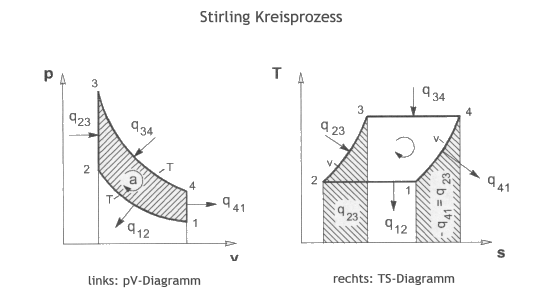
\includegraphics[width = 13cm]{ph_stirlingprozess.png}\\
		& 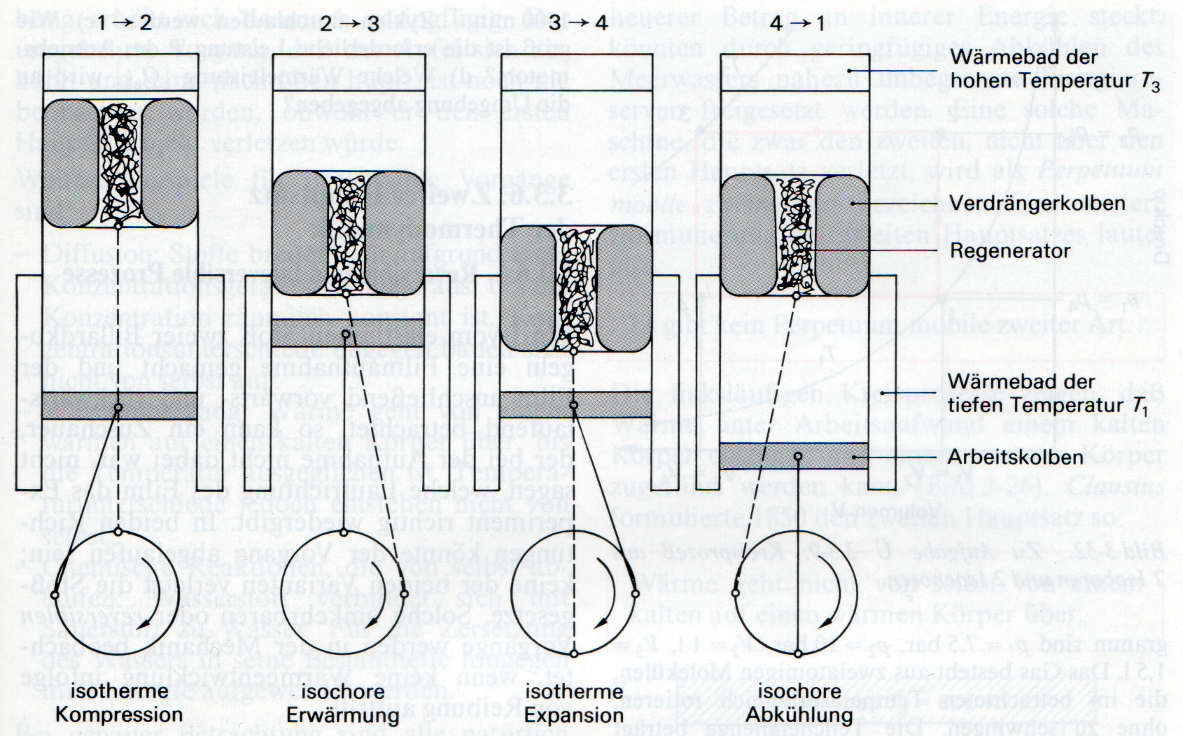
\includegraphics[width = 13cm]{ph_stirlingschema.png}\\
Wirkungsgrad	& $\eta = 1-\frac{T_1}{T_3}$
\end{tabular}\\
\subsubsection{Weitere Prozesse}
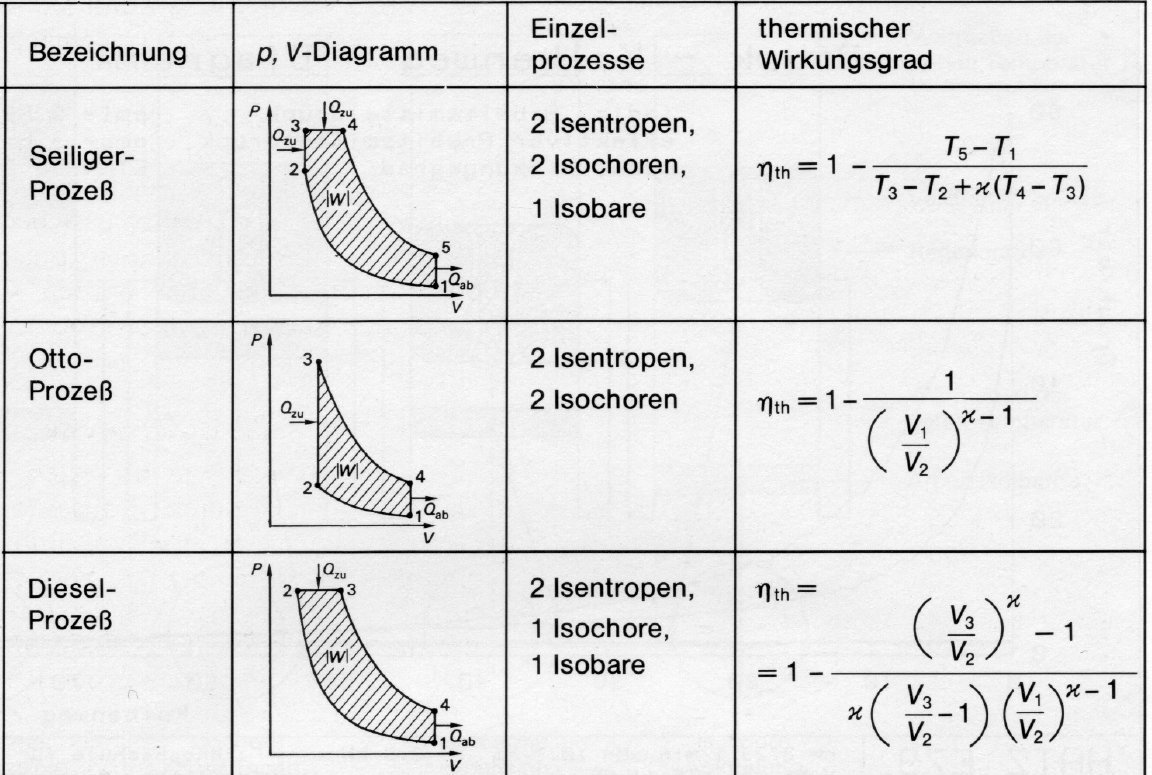
\includegraphics[width = 19cm]{ph_kreisprozesse.png}
\subsubsection{Umgekehrter Kreisprozess}
Aus mechanischer Arbeit wird W�rme oder K�lte gewonnen.\\
\begin{tabular}{p{4cm}p{15cm}}
Leistungszahl	& $\epsilon = \frac{\text{Nutzen}}{\text{Aufwand}}$\\
K�ltemaschine	& $\epsilon_K = \frac{|Q_{zu}|}{W} = \frac{T_1}{T_3 - T_1}$\\
W�rmepumpe	& $\epsilon_W = \frac{|Q_{ab}|}{W} = \frac{T_3}{T_3 - T_1}$
\end{tabular}
\subsection{3. Hauptsatz}
$S$ = 0 oder $T = 0$ l�sst sich nicht erreichen.
%Transportph�nomene (Diffusion u. W�rmeleitung)
\section{Transportph�nomene}
\begin{tabular}[t]{p{4cm}p{15cm}}
mikroskopischer Stossquerschnitt	& $\sigma = 4\pi r^2$\\
mittlere freie Wegl�nge			& $\Lambda = \frac{1}{n\sigma}\quad n:$ Teilchendichte\\
``Teilchenintensit�t''			& $W(L) = ae^{-L/\Lambda}$\\
Absorptionsl�nge			& $l_a \equiv \Lambda_a = \frac{1}{n\sigma_a}$\\
Absorptionskoeffizient			& $\alpha = n\sigma_a\quad$ Anzahl absorbierte Photonen pro L�ngeneinheit\\
Intensit�t des Lichts			& $I(z) = I_0e^{-\alpha z}$
\end{tabular}
\subsection{Diffusion und W�rmeleitung}
\begin{tabular}{p{9.5cm}p{9.5cm}}
\textbf{Diffusion}						& \textbf{W�rmeleitung}\\\midrule
Fick'sches Gesetz (Diffusionsstromdichte)			& Fourier'sches Gesetz (W�rmestromdichte)\\
$\mathbf{j(r)} = -D \textrm{~grad~} n(\boldsymbol{r})$		& $\boldsymbol{j_Q(r)} = -K \textrm{~grad~} T(\boldsymbol{r})$\\\midrule
Diffusionskonstante $[D] = \frac{m^2}{s}$			& W�rmeleitf�higkeit $[K] = \frac{J}{m\cdot s \cdot K} = \frac{W}{m\cdot K}$\\\midrule
f�r Gase und Fl�ssigkeiten					& f�r Gase und Fl�ssigkeiten\\
$D = \frac{1}{3}\langle v \rangle \Lambda$			& $K = D\left( \frac{3}{2}nk_B \right) = \frac{1}{2}nk_B \langle v \rangle \Lambda$\\
$\langle v \rangle = \sqrt{\frac{8 k_BT}{\pi m}}$		& \\\midrule
station�rer Zustand: $j(x) =$ konst.				& station�rer Zustand: $j_Q(x) =$ konst.\\
$n(x) = -\frac{j}{D}x + n_0$					& $T(x) = -\frac{j_Q}{K}x + T_0$\\\midrule
Kontinuit�tsgleichung: Teilchenerhaltung			& Kontinuit�tsgleichung: Energieerhaltung\\
$\frac{\partial n}{\partial t} + \textrm{~div~} \boldsymbol{j} = 0$	& $\frac{\partial \rho_Q}{\partial t} + \textrm{~div~} \boldsymbol{j_Q} = 0$\\\midrule
\textbf{Diffusionsgleichung}					& \textbf{W�rmeleitungsgleichung}\\
$\frac{\partial n(x,t)}{\partial t}-D \nabla^2 n(x,t) = 0$	& $\frac{\partial T(x,t)}{\partial t}-D_W \nabla^2 T(x,t) = 0$\\
								& $D_W \equiv \frac{K}{\rho c}, \rho:$ Massendichte, $c$: spez. W�rmekapazit�t\\\midrule
\multicolumn{2}{l}{Driftstromdichte: $j = n\cdot v_d \cdot f$\quad $f:$ ``generische'' Teilcheneigenschaft, z.B. $f = q$ f�r Ladung}\\
Teilchenstromdichte: $\boldsymbol{j(r)}$ 			& W�rmestromdichte: $\boldsymbol{j_Q(r)}\quad [\boldsymbol{j_Q(r)}] = \frac{J}{m^2\cdot s}$\\
Teilchenstrom: $I = \int_A \boldsymbol{j(r)}dA$			& W�rmestrom: $I_Q = \int_A \boldsymbol{j}_Q(\boldsymbol{r})dA$\\
Teilchendichte: $n(r,t)$					& W�rmedichte: $\rho_Q$
\end{tabular}
\subsection*{Beispiel station�rer Zustand}
W�rmestromdichte in 1D: $j_Q = -K \frac{\partial T(x)}{\partial x}$\\
$dT = -\frac{j_Q}{K}dx \Rightarrow \int_{T_1}^{T(x)}dT = -\frac{j_Q}{K}\int_{x_1}^{x}dx,$ falls $j_Q(r)$ konst.\\
Randbedingungen: $T(x_1) = T_1, T(x_2) = T_2$\\
W�rmestromdichte: $j_Q = -K \frac{T_2-T_1}{x_2-x_1}$\\
Temperaturprofil: $T(x) = T_1 -\frac{j_Q}{K}(x-x_1)$
%Konstanten
\section{Anhang}
\subsection{Grundkonstanten}
\begin{tabular}{p{8cm} p{2cm} p{8cm}}
Konstante			& Symbol	& Wert\\\midrule
Lichtgeschwindigkeit im Vakuum	& $c$		& $2.9979 \cdot 10^8 $m s$^{-1}$\\
Elementarladung			& $e$		& $1.6021 \cdot 10^{-19} $C\\
Ruhemasse des Elektrons		& $m_e$		& $9.1094 \cdot 10^{-31}$kg\\
Ruhemasse des Protons		& $m_p$		& $1.6726 \cdot 10^{-27}$kg\\
Ruhemasse des Neutrons		& $m_n$		& $1.6749 \cdot 10^{-27}$kg\\
Planck'sche Konstante		& $h$		& $6.621 \cdot 10^{-34} $J s\\
				&		& $= 4.135 \cdot 10^{-15} $eV s\\
				& $\hbar = \frac{h}{2\pi}$	& $1.0546 \cdot 10^{-34}$ J s\\
Bohr'scher Radius		& $a_0$		& $5.2918 \cdot 10^{-11}$m\\
Comptonwellenl�nge		&\\
$\quad$ d. Elektrons		& $\lambda_{c,e}$	& $2.4263 \cdot 10^{-12}$m\\
$\quad$ d. Protons		& $\lambda_{c,p}$	& $1.3214 \cdot 10^{-15}$m\\
Rydberg-Konstante		& $R$		& $1.0974 \cdot 10^7 $m$^{-1}$\\
Bohr'sches Magneton		& $\mu_B$	& $9.2740 \cdot 10^{-24} $J T$^{-1}$\\
Avogadro-Konstante		& $N_A$		& $6.0221 \cdot 10^{23} $mol$^{-1}$\\
Boltzmann-Konstante		& $k_B$		& $1.3807 \cdot 10^{-23} $J K$^{-1}$\\
				&		& $= 8.6173 \cdot 10^{-5} $eV K$^{-1}$\\
universelle Gaskonstante	& $R$		& $8.314$ J mol$^{-1}$ K$^{-1}$\\
Stefan-Boltzmann-Konstante	& $\sigma$	& $5.67\cdot 10^{-8} $W m$^{-2}$K$^{-4}$\\
Schwerebeschleunigung in Meeresh�he am �quator	& $g$	& $9.7805 $m s$^{-2}$\\
Atommasse			& $u$		& $1.660 \cdot 10^{-27}$ kg
\end{tabular}
\subsection{Einheiten und Zeichen}
\begin{tabular}{p{8cm} p{2cm} p{4cm} p{4cm}}
Gr�sse			& Symbol	& Bezeichnung der Einheit	& SI-Gr�sse\\\midrule
L�nge			& $l$		& Meter				& m\\
Masse			& $m$		& Kilogramm			& kg\\
Zeit			& $t$		& Sekunde			& s\\
Geschwindigkeit		& $v$		&				& ms$^{-1}$\\
Beschleunigung		& $a$		&				& ms$^{-2}$\\
Winkelgeschwindigkeit	& $\omega$	&				& s$^{-1}$\\
Kreisfrequenz		& $\omega$	&				& s$^{-1}$\\
Frequenz		& $\nu$		& Hertz (Hz)			& s$^{-1}$\\
Impuls			& $p$		&				& m kg s$^{-1}$\\
Kraft			& $F$		& Newton (N)			& m kg s$^{-2}$\\
Druck			& $p$		& Pascal (Pa)			& m$^{-1}$ kg s$^{-2}$\\
Drehimpuls		& $L$		&				& m$^2$ kg s$^{-1}$\\
Drehmoment		& $\tau$	&				& m$^2$ kg s$^{-2}$\\
Arbeit			& $W$		& Joule (J)			& m$^2$ kg s$^{-2}$\\
Leistung		& $P$		& Watt (W)			& m$^2$ kg s$^{-3}$\\
Energie			& $U,E$		& Joule (J)			& m$^2$ kg s$^{-2}$\\
Temperatur		& $T$		& Kelvin (K)			& m$^2$ kg s$^{-2}$ / Teilchen\\
Diffusionskoeffizient	& $D$		&				& m s$^{-2}$\\
W�rmeleitf�higkeit	& $K$		&				& m kg s$^{-3}$ K$^{-1}$\\
Elektrischer Strom	& $I$		& Amp�re (A)			& A\\
Ladung			& $q,Q$		&				& A s\\
Elektrisches Feld	& $\epsilon$	& 				& m kg s$^{-3}$ A$^{-1}$\\
Elektrisches Potential	& $V$		& Volt (V)			& m$^2$ kg s$^{-3}$ A$^{-1}$\\
Stromdichte		& $j$		&				& m$^{-2}$ A\\
Magnetfeld		& $B$		& Tesla (T)			& kg s$^{-2}$ A$^{-2}$\\
\end{tabular}
\subsection{N�tzliche Beziehungen}
\begin{tabular}{p{5cm}p{14cm}}
Elektronenvolt			& $1 $eV$ = 1.602 \cdot 10^{-19}$ J\\
				& $1 $J$ = 6.242 \cdot 10^{18}$ eV\\
Planck'sches Wirkungsquantum	& $hc = 1240 $eV$\cdot nm$\\
Boltzmann-Konstante		& $k_B T = 25.8 $ meV $ ($at $T=300 K) = 4.133 \cdot 10^{-21}J$\\
Temperatur			& K = 273.15 + $^{\circ}$C\\
Bar - Pascal			& 1 bar = $10^5$ Pa\\
Coulomb - Ampere		& C = A s
\end{tabular}\\
\begin{tabular}{lcl|p{15cm}}
Energie $E = \hbar\omega$	& $\Leftrightarrow$	& Wellenl�nge $\lambda$	& $E [eV] = \frac{1.24}{\lambda[\mu m]}$\\
Frequenz $\nu$			& $\Leftrightarrow$	& reduzierte Wellenzahl $\frac{1}{\lambda}$	& $\nu[GHz] = \frac{30}{\lambda}\left[cm^{-1}\right]$\\
Kreisfrequenz $\omega$		& $\Leftrightarrow$	& Wellenzahl $k$	& $\omega[GHz] = 30 \cdot k \left[cm^{-1}\right]$
\end{tabular}
\subsection{Koordinatensysteme}
\subsubsection{Polarkoordinaten}
\begin{tabular}{p{4cm} p{15cm}}
Definition	& $\begin{array}[t]{l}
                	  x = r \cdot \sin \varphi\\
			  y = r \cdot \cos \varphi\\
                	 \end{array}$\\
Gradient	& $\nabla f= \frac{\partial f}{\partial r } \vec{e}_r +  \frac{1}{r} \frac{\partial f}{\partial \varphi} \vec{e}_\varphi$\\
Laplace		& $\Delta f(r, \varphi ) =
\frac{\partial^2 f}{\partial r^2} +
\frac{1}{r}\frac{\partial f}{\partial r} +
\frac{1}{r^2}\frac{\partial^2 f}{\partial \varphi^2}$\\
oder		& $\Delta f(r, \varphi ) =
\frac{1}{r}\frac{\partial}{\partial r}
\left( r\,\frac{\partial f}{\partial r} \right) +
\frac{1}{r^2}\frac{\partial^2 f}{\partial \varphi^2}$\\
Volumenelement	& d$x$ d$y$ = $r$ d$\varphi$ d$r$
\end{tabular}
\subsubsection{Zylinderkoordinaten}
\begin{tabular}{p{4cm} p{15cm}}
Definition	& $\begin{array}[t]{l}
                	  x = r \cdot \sin \varphi\\
			  y = r \cdot \cos \varphi\\
			  z = z
                	 \end{array}$\\
Gradient	& $\nabla f= \frac{\partial f}{\partial r } \vec{e}_r +  \frac{1}{r} \frac{\partial f}{\partial \varphi} \vec{e}_\varphi+ \frac{\partial f}{\partial z} \vec{e}_z $\\
Laplace		& $\Delta f ( r , \varphi , z ) = \frac{1}{r} \frac{\partial}{\partial r}
\left( r\,\frac{\partial f}{\partial r} \right) +
\frac{1}{r^2}\frac{\partial^2 f}{\partial \varphi^2} +
\frac{\partial^2 f}{\partial z^2}$\\
Volumenelement	& d$x$ d$y$ d$z$ = $r$ d$z$ d$\varphi$ d$r$
\end{tabular}
\subsubsection{Kugelkoordinaten}
\begin{tabular}{p{4cm} p{15cm}}
Definition		&$\begin{array}[t]{l}
                	  x = r \cdot \sin \theta \cdot \cos \varphi\\
			  y = r \cdot \sin \theta \cdot \sin \varphi\\
			  z = r \cdot \cos \theta
                	 \end{array}$\\
Gradient		& $\mathbf{\nabla}
  =\mathbf{e}_r\frac{\partial}{\partial r} 
   + \mathbf{e}_\theta\frac{1}{r}\frac{\partial}{\partial\theta}
   + \mathbf{e}_\varphi\frac{1}{r\sin\theta}\frac{\partial}{\partial\varphi}$\\
Laplace			& $\Delta f ( r , \theta , \varphi ) = \frac{1}{r^2} 
\frac{\partial}{\partial r} \left( r^2  \,\frac{\partial f}{\partial r} \right) +
\frac{1}{r^2 \sin \theta}  \frac{\partial}{\partial \theta} \left(\sin\theta \, \frac{\partial f}{\partial \theta} \right) +
\frac{1}{r^2 \sin^2\theta}  \frac{\partial^2 f}{\partial \varphi^2}$\\
Volumenelement		& d$x$ d$y$ d$z$ = $r^2 \sin \theta $ d$\varphi$ d$\theta$d$r$
\end{tabular}

\subsection{Trigonometrische Identit�ten und Integrale}
\subsubsection{Identit�ten}
\begin{tabular}{ll}
$\sin(a \pm b) = \sin a \cos b \pm \cos a \sin b$	& $\sin a \sin b = \frac{1}{2} \left( \cos(a-b) - \cos (a + b) \right)$\\
$\cos(a \pm b) = \cos a \cos b \mp \sin a \sin b$	& $\cos a \cos b = \frac{1}{2} \left( \cos(a-b) + \cos (a + b) \right)$\\
$\sin^2(x) = -\frac{\cos(2x)}{2} + \frac{1}{2}$		& $\sin a \cos b = \frac{1}{2} \left( \sin(a-b) + \sin (a + b) \right)$\\
$\cos^2(x) = \frac{\cos(2x)}{2} + \frac{1}{2}$		& $\sin(2x) = 2\sin(x) \cos(x)$\\
							& $\cos(2x) = \cos^2(x)-\sin^2(x)$
\end{tabular}

\subsubsection{Integrale}
$
\begin{array}{ll}
\int \sin^2(ax) dx = \frac{x}{2}  - \frac{1}{4a} \sin(2ax)			& \int \sin^3(ax) dx = -\frac{1}{a} \cos(ax) + \frac{1}{3a} \cos^3(ax)\\
\int x \cdot \sin(ax) dx = \frac{1}{a^2} \sin(ax) - \frac{x}{a} \cos(ax)	& \int x^2 \sin(ax) dx = \frac{2x}{a^2} \sin(ax) - \frac{x^2}{a} \cos(ax) + \frac{2}{a^3}\cos(ax)\\
\int \cos^2(ax) dx = \frac{x}{2}  + \frac{1}{4a} \sin(2ax)			& \int \cos^3(ax) dx = -\frac{1}{a} \cos(ax) - \frac{1}{3a} \sin^3(ax)\\
\int x \cdot \cos(ax) dx = \frac{1}{a^2} \cos(ax) + \frac{x}{a} \sin(ax)	& \int x^2 \cos(ax) dx = \frac{2x}{a^2} \cos(ax) + \frac{x^2}{a} \sin(ax) - \frac{2}{a^3}\sin(ax)\\
\int x \cdot \sin^2(ax) dx = -\frac{2ax (\sin(2ax)-ax) + \cos(2ax)}{8a^2}

\end{array}
$
\subsection{Eigenschaften gerader und ungerader Funktionen}
\begin{itemize}
\item $f(g(x))$ ist gerade, falls $g(x)$ gerade ist. $f(x)$ beliebig. Z.B. $\sin(x^2)$
\item $f(g(x))$ ist gerade, falls $g(x)$ ungerade und $f(x)$ gerade. Z.B. $\sin^2(x)$
\item $f(g(x))$ ist ungerade, falls $g(x)$ ungerade und $f(x)$ ungerade. Z.B. $\sin^3(x)$
\item Cosinus ist gerade, Sinus ist ungerade.
\item Die Ableitung einer geraden Funktion ist ungerade, die Ableitung einer ungeraden Funktion ist gerade.
\item Die Fourierreihe einer geraden (ungeraden) Funktion enth�lt nur Cosinus - (Sinus-) Terme.
\end{itemize}

\subsection{Genaue Funktionswerte}
$
\begin{array}{l|ccccccccc}
 \alpha		& 0	& \frac{\pi}{6}		& \frac{\pi}{4}		& \frac{\pi}{3}		& \frac{\pi}{2}	& \frac{2\pi}{3}	& \frac{3\pi}{4}	& \frac{5\pi}{6}	& \pi\\\hline
 \sin\alpha	& 0	& \frac{1}{2}		& \frac{\sqrt{2}}{2}	& \frac{\sqrt{3}}{2}	& 1		& \frac{\sqrt{3}}{2}	& \frac{\sqrt{2}}{2}	& \frac{1}{2}		& 0\\
 \cos\alpha	& 1	& \frac{\sqrt{3}}{2}	& \frac{\sqrt{2}}{2}	& \frac{1}{2}		& 0		& -\frac{1}{2}		& -\frac{\sqrt{2}}{2}	& -\frac{\sqrt{3}}{2}	& -1\\
 \tan\alpha	& 0	& \frac{\sqrt{3}}{3}	& 1			& \sqrt{3}		& -		& -\sqrt{3}		& -1			& -\frac{\sqrt{3}}{3}	& 0\\
\end{array}\\
$

\subsection{Fourierreihen}
\subsubsection{Definition}
 Lipstetige T-periodische Funktionen $( f(t) = f(t+T) )$ lassen sich als trigonometrische Reihe darstellen
\begin{equation*}
 f(t) = \frac{a_0}{2} + \sum_{n=1}^{\infty} \left(a_n \cos\left(\frac{2\pi}{T} nt \right) + b_n \sin\left(\frac{2\pi}{T} nt \right) \right)
\end{equation*}
mit reellen Koeffizienten $a_n, b_n$ oder wie folgt:
\begin{equation*}
 f(t) = \sum_{n=-\infty}^{\infty} c_n e^{\frac{2\pi i}{T} nt},\quad c_n\in\mathbb{C}
\end{equation*}
mit komplexen Koeffizienten $c_n$\\
\subsubsection{Bestimmung der Koeffizienten}
$c_n = \frac{1}{2} (a_n -ib_n)\\
c_{-n} = \frac{1}{2} (a_n +ib_n) = \overline{c_n}\\
c_0 = \frac{1}{2} a_0\\\\
c_n = \frac{1}{T} \int_{-T/2}^{T/2} f(t)\cdot e^{\frac{-2\pi i}{T}nt} dt\\
a_n = \left(c_n + c_{-n}\right) = \frac{2}{T} \int_{-T/2}^{T/2} f(t) \cos\left(\frac{2\pi}{T}nt \right) dt\\
b_n = \left(\frac{c_n - c_{-n}}{i}\right) =  \frac{2}{T} \int_{-T/2}^{T/2} f(t) \sin\left(\frac{2\pi}{T}nt \right) dt$\\\\
Falls $f$ gerade $\Leftrightarrow f(t) = f(-t)$, dann $b_n = 0 \forall n$\\
Falls $f$ ungerade $\Leftrightarrow f(-t) = -f(t)$, dann $a_n = 0 \forall n$\\

\subsection{Fouriertransformation (FT)}
 \begin{align*}
 \text{FT} := &\hat{f}(\omega) = \int_{-\infty}^{\infty} f(t)e^{-i\omega t} dt\quad \omega\in\mathbb{R}\\
	  &f(t) = \frac{1}{2\pi} \int_{-\infty}^{\infty} \hat{f}(\omega) e^{i\omega t} d\omega
\end{align*}
$
\begin{array}{lll}
 \text{Linearit�t:} 	&h(t) = af(t) + bg(t)			&\Rightarrow \hat{h}(t) = a\hat{f}(t) + b\hat{g}(t)\\
 \text{Verschiebung:}	&g(t) = f(t-a)				&\Rightarrow \hat{g}(\omega) = e^{-ia\omega} \hat{f}(\omega)\\
 			&g(t) = e^{iat}f(t)			&\Rightarrow \hat{g}(\omega) = \hat{f}(\omega-a)\\
 \text{Skalierung:}	&g(t) = f\left(\frac{t}{a}\right) (a>0)	&\Rightarrow \hat{g}(\omega) = a\hat{f}(a\omega)\\
 \text{Ableitung:} 	&g(t) = f'(t)				&\Rightarrow \hat{g}(\omega) = i\omega\hat{f}(\omega)\\
 \text{Faltungsprodukt:}& \multicolumn{2}{l}{\text{Definition im ``Fourierraum'':} \Bigl( f\ast g\Bigr)(t) := \int_{-\infty}^{\infty} f(t-s)g(s) ds}\\
			&\Bigl(f\ast g\Bigr)(t)			&\Rightarrow \widehat{f\ast g} (\omega) = \hat{f}(\omega)\cdot \hat{g}(\omega)\\
 \text{Standard-FT:}	&f(t) = e^{-\frac{at^2}{2}}\quad a>0	&\Rightarrow \hat{f}(\omega) = \sqrt{\frac{2\pi}{a}} e^{\frac{-\omega^2}{2a}}
\end{array}
$

\end{document}